\documentclass[notes]{beamer}
\usepackage{pgfpages}
\usepackage{amsmath}
\usepackage{graphicx}
\usepackage{subfig}
\usepackage{tikz}
\usepackage{pgfplots}
\usepackage[style=verbose]{biblatex} 
\setbeameroption{show notes on second screen=right}
\makeatletter
\let\@@magyar@captionfix\relax
\makeatother

\bibliography{../link.bib}
\renewcommand{\footnotesize}{\tiny}
\title{Latent Variable Machine Learning Algorithms: Applications in a Nuclear Physics Experiment
}
\author{Robert Solli}
\institute{University of Oslo, Expert Analytics AS}
\date{\today}

\begin{document}
\begin{frame}[t]{Thesis Presentation}
	\titlepage
\end{frame}

\begin{frame}[t]{Outline}
	\begin{enumerate}
		\item Introducing the Active Target Time Projection Chamber (AT-TPC)
		\item Challenges with traditional analysis of AT-TPC data - and the evangilization of Machine Learning
			\begin{enumerate}[(i)]
				\item Recap of central literature 
				\item Introducing thesis problem statements
			\end{enumerate}
		\item An introduction to central Machine Learning concepts
		\item The Auto-Encoder neural network
		\item Results 
		\item Summary, Conclusion and Outlook
	\end{enumerate}
\end{frame}

\begin{frame}[t]{AT-TPC}
	\begin{figure}
		\centering
		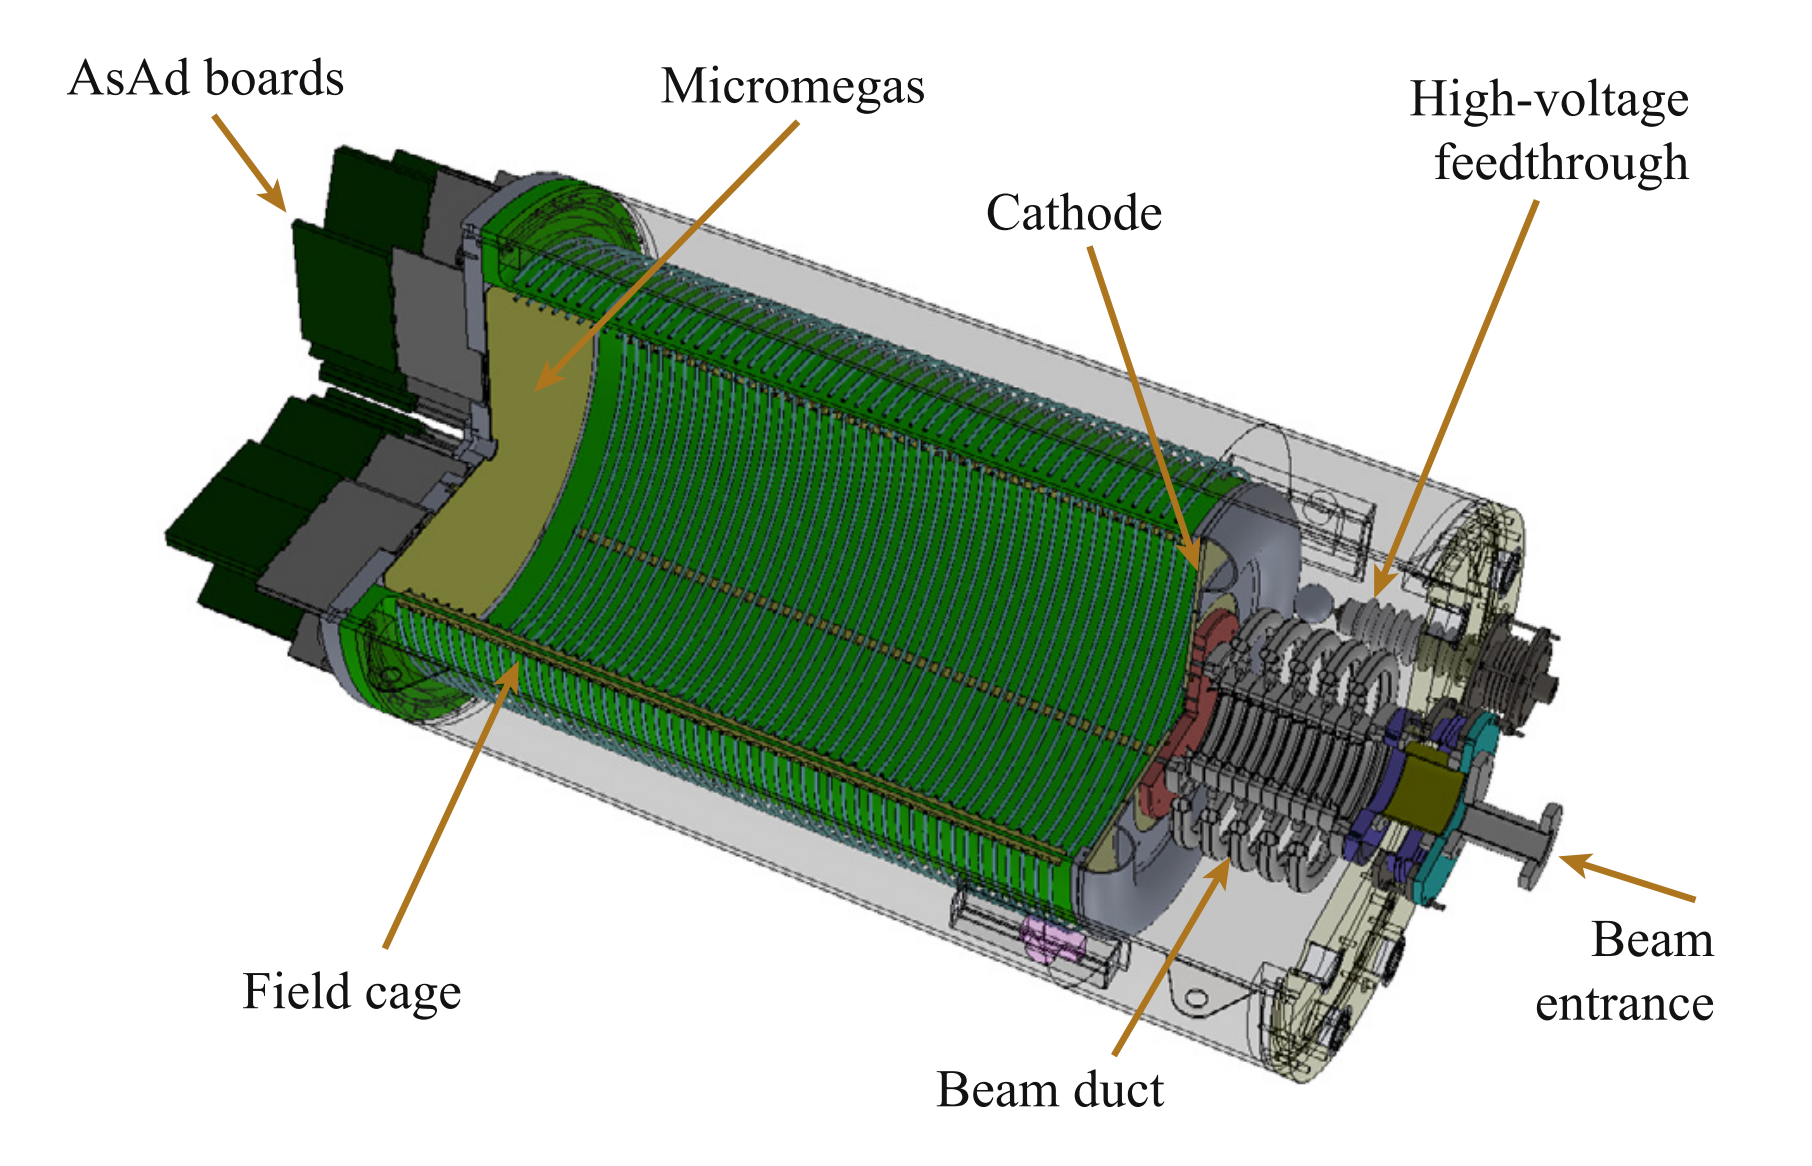
\includegraphics[height=3cm]{../chapters/experimental_background/plots/at_tpc_schematic.png}
		\caption{Diagram of the AT-TPC \footcite{Bradt2017a}}\label{fig:attpc}
	\end{figure}
	The AT-TPC is an experiment set up at the rare isotopes facility on the Michigan State University campus. The AT-TPC is commissioned to capture reactions with exotic nuclei.
\end{frame}
\note{
	$1e4$ pads, $1e2$ timebuckets, $1e5$ events/hr: terrabytes of data.
}

\begin{frame}[t]{AT-TPC Data}
	\begin{figure}[t]
		\centering
		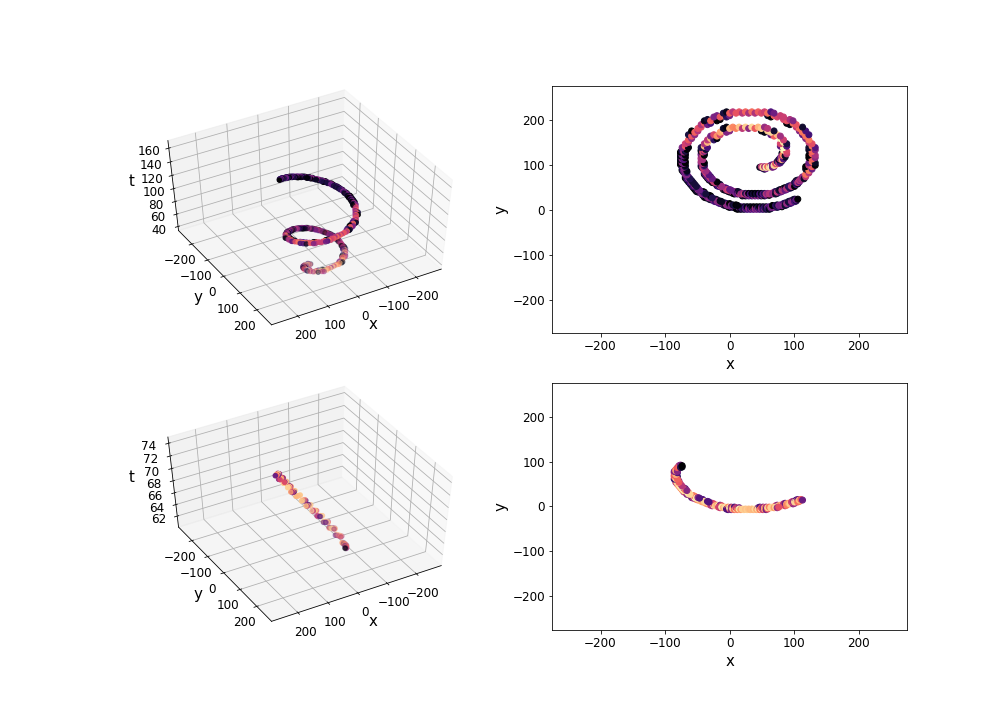
\includegraphics[width=0.8\linewidth]{../chapters/experimental_background/plots/display_eventssimulated.png}
		\caption{Simulated AT-TPC data top row: a proton trajectory, bottom row: a carbon trajectory}
		\label{fig:name}
	\end{figure}
\end{frame}

\note{
	Remember: talk about the plots in detail.
	Proton on top, carbon on bottom.

	Reactions in the whole volume (development of spirals), spirals from magnet.
}

\begin{frame}[t]{AT-TPC Data}
	\begin{figure}
		\subfloat[Unfiltered events AT-TPC. Top: carbon nucleus, bottom: proton]{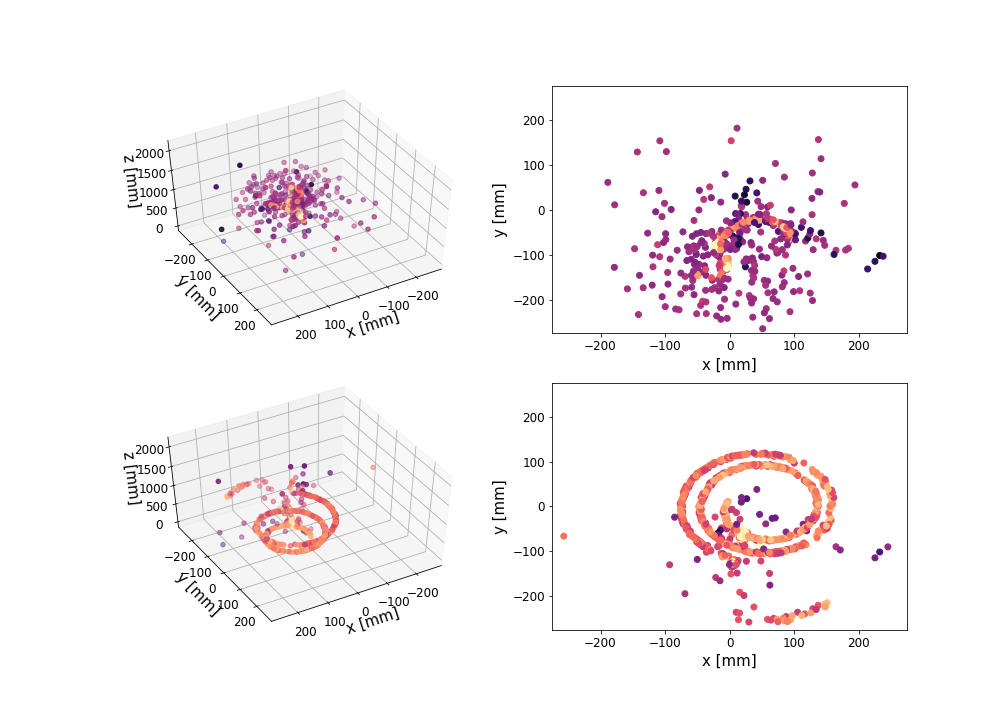
\includegraphics[width=0.4\linewidth]{../chapters/experimental_background/plots/display_eventsfull_.png}}
		\subfloat[Same events as in (a), but filtered]{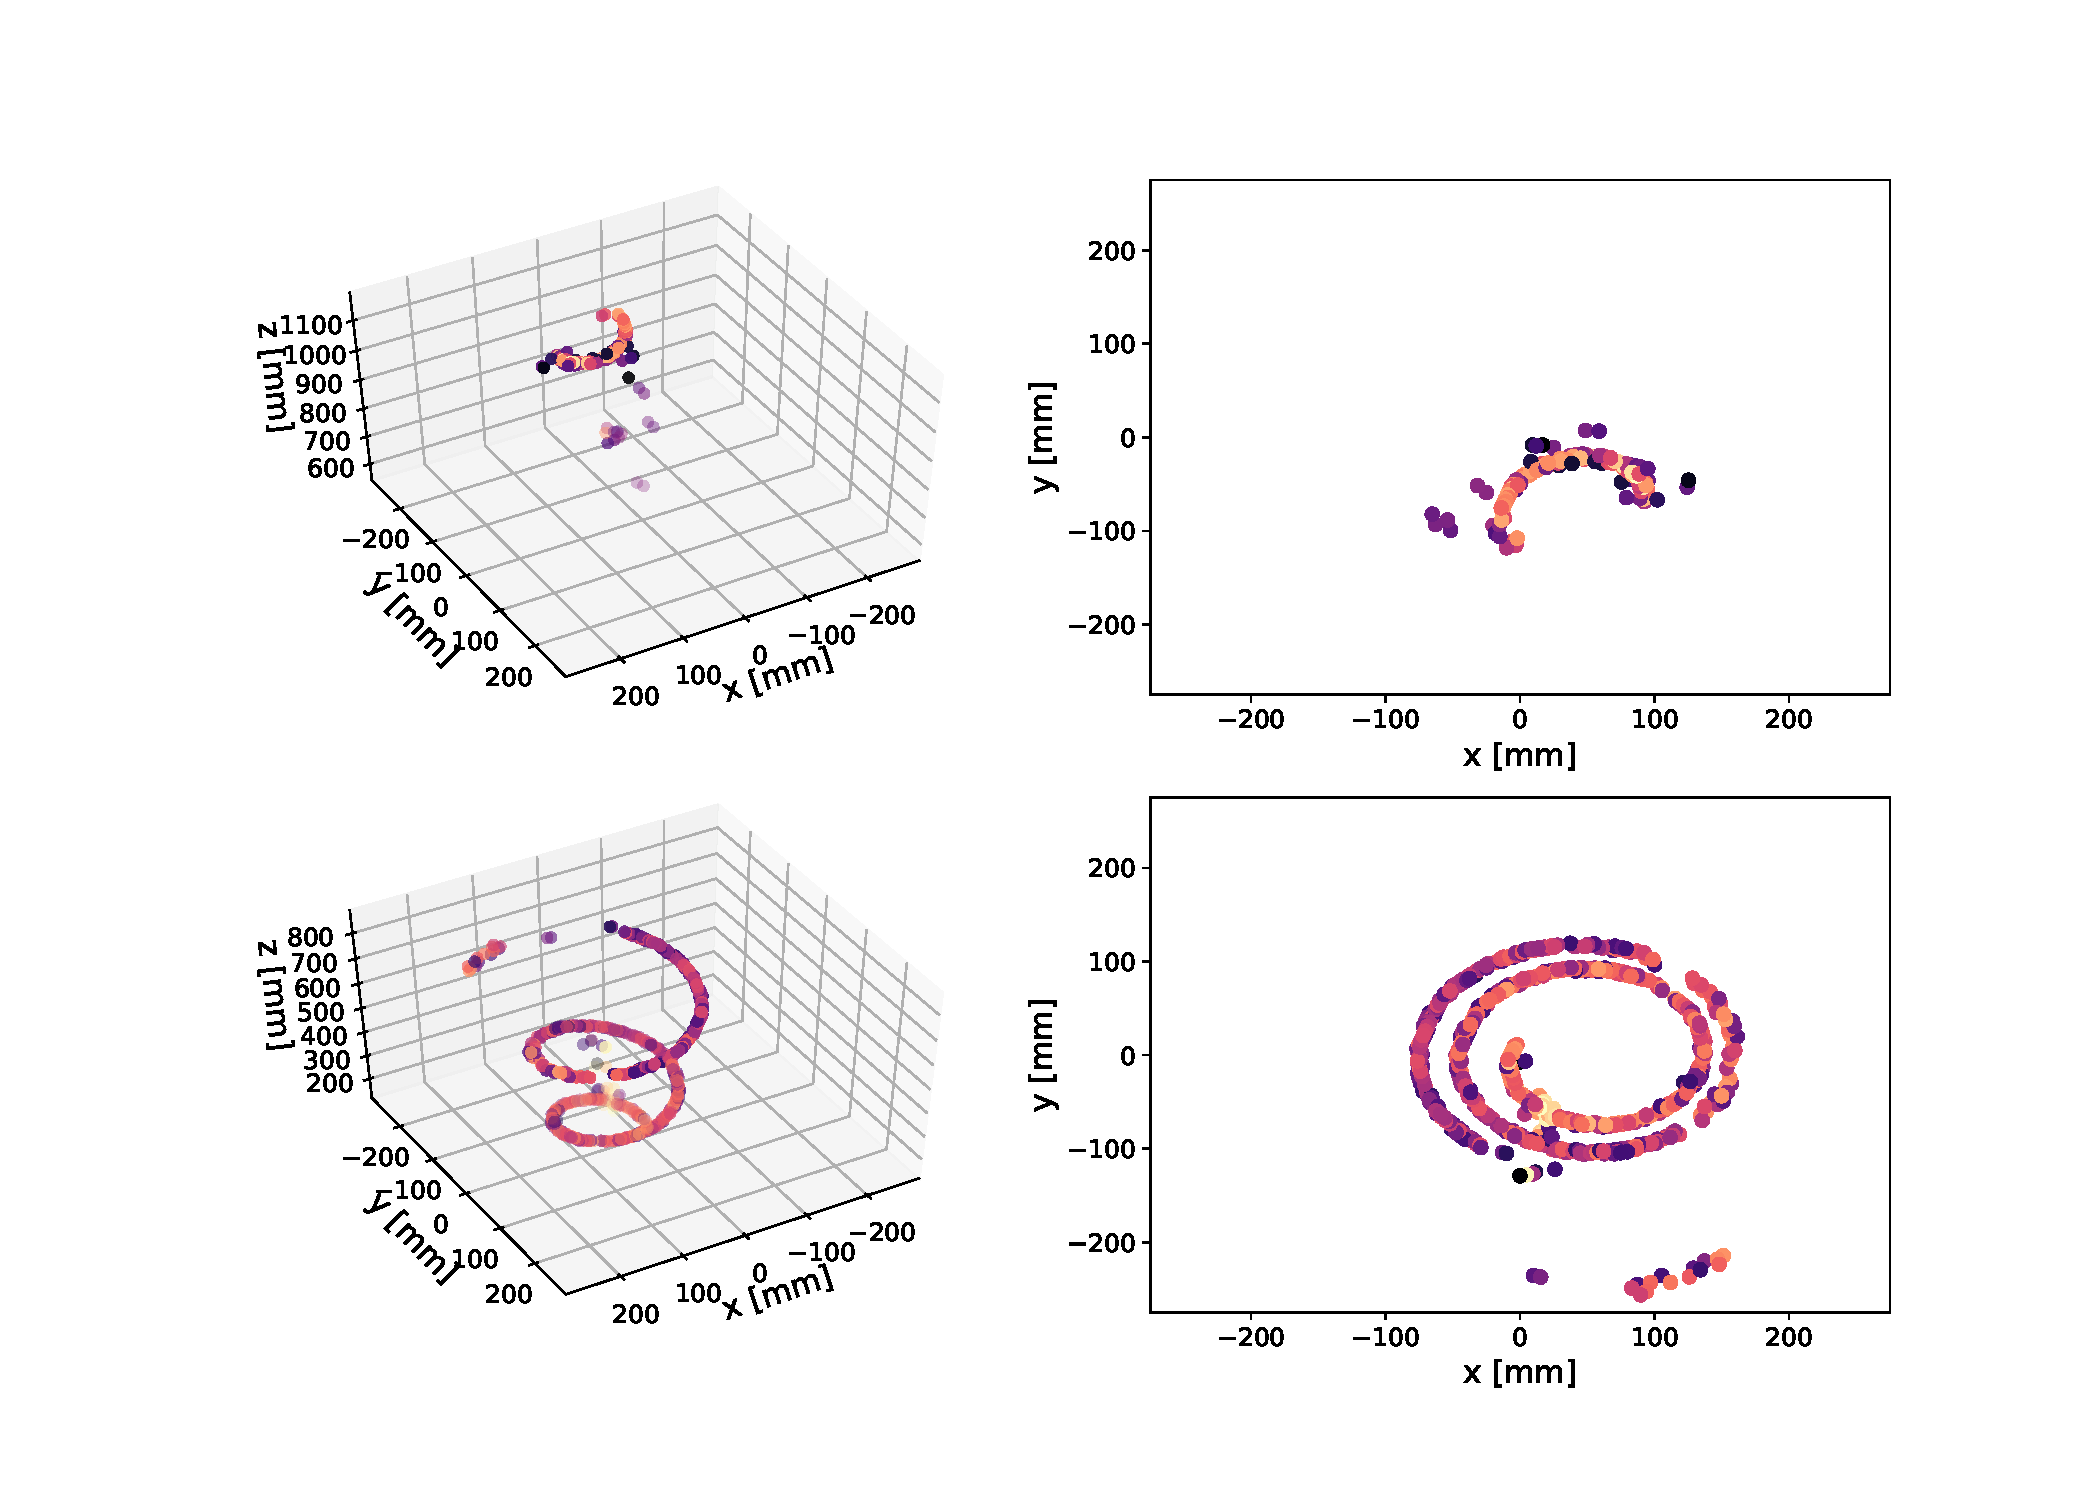
\includegraphics[width=0.5\linewidth]{../chapters/experimental_background/plots/display_eventsclean_.pdf}}
	\end{figure}
	Significant noise levels in the experiment, from unknown sources. Some $60\%$ of the recorded events are from unidentified reactions.
\end{frame}

\note{
	Remember - talk about event plots in detail.\\
	Not pictured: pure noise events.\\
	More noise in carbon - more ionizing: not necessarily uncorrelated noise \\

	\begin{enumerate}[I]
			\item Expensive integration - for each event a fit is computed.
			\item Assumptions of the integration technique: 
				\begin{enumerate}[(i)]
					\item Each event is fit against parameters of the event of interest,
					\item The integration is sensitive to Noise and Breaks in the tracks.
				\end{enumerate}
			\item In some experiments researchers are unable to identify samples of the positive class of events.
	\end{enumerate}
}

\begin{frame}[t]{Challenges with the AT-TPC}
	\begin{enumerate}[I]
		\item Expensive integration - for each event a fit is computed.
		\item Assumptions of the integration technique: 
			\begin{enumerate}[(i)]
				\item Each event is fit against parameters of the event of interest,
				\item The integration is sensitive to Noise and Breaks in the tracks.
			\end{enumerate}
		\item In some experiments researchers are unable to identify samples of the positive class of events.
	\end{enumerate}
	The amount of data is also significant: the experiment generates on the order of $10^5$ events per hour running.
	\begin{block}{Idea}
		Solve the problem by training deep neural networks.
	\end{block}
\end{frame}

\begin{frame}[t]{Previous Work}
	\begin{itemize}
		\item Work on applying ML to this data started with a supervised learning project by Kuchera et al.\footcite{Kuchera2019}.
		\item By fine tuning pre-trained networks the authors achieve very impressive performance.
	\end{itemize}
	One of the open questions is then, can we segment the events based on reactions without the ground truth labels?
\end{frame}

\note{
	The authors explored a \textit{supervised classification} problem of identifying reactions when ground-truth labels available.
}


\begin{frame}[t]{Why machine learning}
	\begin{enumerate}[I]
		\item Modern computing resources have created a resurgence in ML fostering strong results in other fields.
		\item Very strong results on image-like data. The resurgence brought Convolutional Neural Networks to the forefront.
		\item Agnostic models can be applied to source data, possibly avoiding biases from filtering.
		\item Broader perspective on what role ML has in (nuclear) physics?
	\end{enumerate}
\end{frame}

\begin{frame}[t]{Machine Learning Principles}
	The ingredients necessary to solve a Machine Learning problem: 
	\begin{enumerate}[(a)]
		\item a model,
		\item datasets,
		\item and a cost function
	\end{enumerate}

	Separate between supervised and unsupervised learning.
\end{frame}

\note{
Cost function measures the quality of the model. \\
Can be MSE, crossent.
}

%\begin{frame}[t]{Deep Learning}
%	Models can be tuned with gradient methods, the simplest of which is a steepest descent update: 
%	\begin{equation}
%		\theta_i \leftarrow \theta_i - \eta \frac{\partial \mathcal{C}(\mathbf{x}, f, \hat{f})}{\partial \theta_i},
%	\end{equation}
%	moderated by a \textit{learning rate} $\eta$ to ensure that the steps are small enough.
%
%	The functional $\mathcal{C}$ is the \textit{cost} function for the problem and is commonly a variation of either, the Mean Squared Error: 
%
%	\begin{equation}
%		\mathcal{C}(\mathbf{x}, f, \hat{f}) = \sum (f(\mathbf{x})_i - \hat{f}(\mathbf{x})_i)^2,
%	\end{equation}
%
%	or the Cross Entropy
%
%	\begin{equation}
%		\mathcal{C}(\mathbf{x}, f, \hat{f}) = -\sum f(\mathbf{x})_i \log \hat{f}(\mathbf{x})_i. 
%	\end{equation}
%\end{frame}

\begin{frame}[t]{Training Neural Networks}
	\begin{figure}[h]
		\centering
		\includegraphics[width=0.6\linewidth]{../chapters/theory/figures/gd_good.pdf}
		\caption{Gradient descent on a quadratic function}
		\label{fig:gd}
	\end{figure}

	Training neural networks is achieved with stochastic gradient methods.
	The function to be optimized is the cost: measuring the quality of the current state of the network.
\end{frame}

\begin{frame}[t]{Deep Learning: Neural Networks}
	\begin{figure}[h]
		\centering
		\includegraphics[width=0.4\linewidth]{../chapters/theory/figures/ann.pdf}
		\caption{A neural network with three input nodes, two hidden nodes, and one output node}
		\label{fig:ann}
	\end{figure}
	Output is computed by passing input forwards through the network to the desired output type.
\end{frame}

\begin{frame}[t]{Hazards in Training}
	\centering
	% This file was created by tikzplotlib v0.8.1.
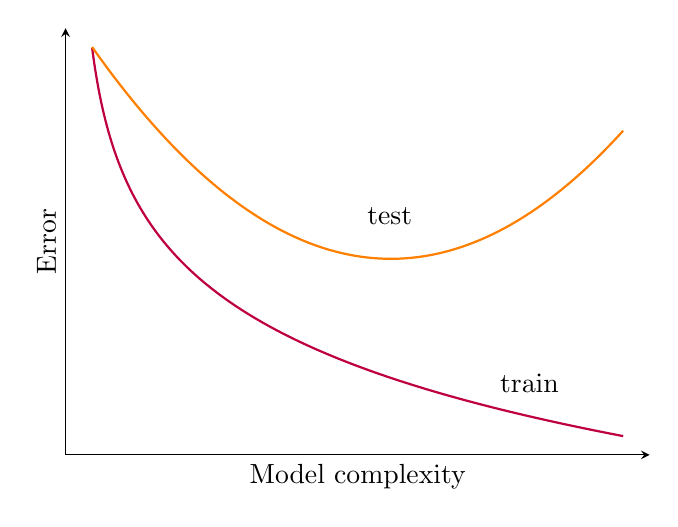
\begin{tikzpicture}

\begin{axis}[
height=7cm, 
width=9cm,
ticks=none,
ylabel near ticks,
xlabel near ticks,
axis x line=bottom,
axis y line=left,
xlabel={Model complexity},
xmin=-0.2, xmax=4.2,
ylabel={Error},
ymin=-16, ymax=4.4
]
\addplot [thick, purple]
table {%
0 3.46573590279973
0.004004004004004 3.26943984054636
0.00800800800800801 3.08055996975182
0.012012012012012 2.89855625448287
0.016016016016016 2.72294557934374
0.02002002002002 2.55329402090492
0.024024024024024 2.38921038789678
0.028028028028028 2.23034078814828
0.032032032032032 2.07636403245592
0.036036036036036 1.92698772528678
0.04004004004004 1.78194492271509
0.044044044044044 1.64099126160566
0.048048048048048 1.5039024824885
0.0520520520520521 1.37047228306363
0.0560560560560561 1.24051045075361
0.0600600600600601 1.11384123187272
0.0640640640640641 0.990301902323346
0.0680680680680681 0.86974151065479
0.0720720720720721 0.752019769128248
0.0760760760760761 0.637006072354703
0.0800800800800801 0.524578626289829
0.0840840840840841 0.414623673020889
0.0880880880880881 0.307034798975167
0.0920920920920921 0.201712316003994
0.0960960960960961 0.0985627063197901
0.1001001001001 -0.00250187645950529
0.104104104104104 -0.101564056829782
0.108108108108108 -0.198701643247571
0.112112112112112 -0.293987995299001
0.116116116116116 -0.387492356531543
0.12012012012012 -0.479280156731312
0.124124124124124 -0.56941328695128
0.128128128128128 -0.657950350185927
0.132132132132132 -0.744946890235164
0.136136136136136 -0.830455600995881
0.14014014014014 -0.914526518155979
0.144144144144144 -0.997207195037107
0.148148148148148 -1.07854286413346
0.152152152152152 -1.15857658572056
0.156156156156156 -1.23734938475645
0.16016016016016 -1.31490037716496
0.164164164164164 -1.39126688647413
0.168168168168168 -1.46648455168055
0.172172172172172 -1.54058742711986
0.176176176176176 -1.61360807504394
0.18018018018018 -1.68557765153477
0.184184184184184 -1.75652598632236
0.188188188188188 -1.82648165701839
0.192192192192192 -1.89547205822808
0.196196196196196 -1.96352346595855
0.2002002002002 -2.03066109770255
0.204204204204204 -2.09690916854147
0.208208208208208 -2.16229094358001
0.212212212212212 -2.22682878699652
0.216216216216216 -2.29054420796793
0.22022022022022 -2.3534579037051
0.224224224224224 -2.41558979981415
0.228228228228228 -2.47695908818075
0.232232232232232 -2.53758426255738
0.236236236236236 -2.59748315201897
0.24024024024024 -2.65667295243809
0.244244244244244 -2.71517025611884
0.248248248248248 -2.77299107971722
0.252252252252252 -2.83015089056543
0.256256256256256 -2.88666463150847
0.26026026026026 -2.94254674435266
0.264264264264264 -2.9978111920183
0.268268268268268 -3.05247147948138
0.272272272272272 -3.10654067358286
0.276276276276276 -3.1600314217784
0.28028028028028 -3.21295596989563
0.284284284284284 -3.26532617896149
0.288288288288288 -3.31715354115734
0.292292292292292 -3.36844919495566
0.296296296296296 -3.41922393948816
0.3003003003003 -3.4694882481916
0.304304304304304 -3.51925228177457
0.308308308308308 -3.5685259005453
0.312312312312312 -3.61731867613791
0.316316316316316 -3.66563990267206
0.32032032032032 -3.71349860737847
0.324324324324324 -3.76090356072069
0.328328328328328 -3.80786328604159
0.332332332332332 -3.85438606876101
0.336336336336336 -3.90047996514947
0.34034034034034 -3.9461528107011
0.344344344344344 -3.99141222812768
0.348348348348348 -4.03626563499401
0.352352352352352 -4.08072025101391
0.356356356356356 -4.12478310502471
0.36036036036036 -4.16846104165712
0.364364364364364 -4.21176072771623
0.368368368368368 -4.25468865828859
0.372372372372372 -4.29725116258944
0.376376376376376 -4.33945440956306
0.38038038038038 -4.38130441324873
0.384384384384384 -4.4228070379241
0.388388388388388 -4.46396800303669
0.392392392392392 -4.50479288793421
0.396396396396396 -4.54528713640318
0.4004004004004 -4.58545606102536
0.404404404404404 -4.6253048473605
0.408408408408408 -4.66483855796373
0.412412412412412 -4.70406213624542
0.416416416416416 -4.74298041018076
0.42042042042042 -4.78159809587608
0.424424424424424 -4.8199198009986
0.428428428428428 -4.85795002807559
0.432432432432432 -4.89569317766909
0.436436436436436 -4.93315355143176
0.44044044044044 -4.97033535504894
0.444444444444444 -5.00724270107231
0.448448448448448 -5.04387961164958
0.452452452452452 -5.08025002115501
0.456456456456456 -5.11635777872485
0.46046046046046 -5.15220665070197
0.464464464464464 -5.18780032299342
0.468468468468468 -5.22314240334467
0.472472472472472 -5.25823642353409
0.476476476476476 -5.29308584149087
0.48048048048048 -5.32769404333971
0.484484484484485 -5.36206434537519
0.488488488488488 -5.39619999596878
0.492492492492492 -5.43010417741113
0.496496496496497 -5.4637800076924
0.500500500500501 -5.49723054222297
0.504504504504504 -5.53045877549701
0.508508508508508 -5.56346764270112
0.512512512512513 -5.59626002127021
0.516516516516517 -5.62883873239272
0.520520520520521 -5.6612065424671
0.524524524524524 -5.69336616451144
0.528528528528528 -5.72532025952805
0.532532532532533 -5.75707143782478
0.536536536536537 -5.78862226029455
0.540540540540541 -5.81997523965481
0.544544544544544 -5.85113284164842
0.548548548548549 -5.88209748620729
0.552552552552553 -5.9128715485802
0.556556556556557 -5.94345736042618
0.560560560560561 -5.97385721087461
0.564564564564565 -6.0040733475533
0.568568568568569 -6.03410797758569
0.572572572572573 -6.06396326855826
0.576576576576577 -6.09364134945928
0.580580580580581 -6.1231443115898
0.584584584584585 -6.15247420944799
0.588588588588589 -6.18163306158758
0.592592592592593 -6.21062285145156
0.596596596596597 -6.23944552818176
0.600600600600601 -6.2681030074052
0.604604604604605 -6.29659717199816
0.608608608608609 -6.32492987282845
0.612612612612613 -6.35310292947687
0.616616616616617 -6.38111813093843
0.620620620620621 -6.40897723630402
0.624624624624625 -6.43668197542321
0.628628628628629 -6.4642340495488
0.632632632632633 -6.49163513196364
0.636636636636637 -6.5188868685905
0.640640640640641 -6.54599087858526
0.644644644644645 -6.57294875491421
0.648648648648649 -6.59976206491584
0.652652652652653 -6.62643235084764
0.656656656656657 -6.65296113041839
0.660660660660661 -6.67934989730643
0.664664664664665 -6.7056001216643
0.668668668668669 -6.73171325061022
0.672672672672673 -6.75769070870678
0.676676676676677 -6.78353389842725
0.680680680680681 -6.80924420060999
0.684684684684685 -6.83482297490112
0.688688688688689 -6.86027156018595
0.692692692692693 -6.88559127500957
0.696696696696697 -6.91078341798675
0.700700700700701 -6.93584926820161
0.704704704704705 -6.96079008559731
0.708708708708709 -6.98560711135605
0.712712712712713 -7.01030156826974
0.716716716716717 -7.03487466110151
0.720720720720721 -7.05932757693839
0.724724724724725 -7.08366148553546
0.728728728728729 -7.10787753965154
0.732732732732733 -7.13197687537695
0.736736736736737 -7.15596061245329
0.740740740740741 -7.17982985458564
0.744744744744745 -7.20358568974734
0.748748748748749 -7.22722919047752
0.752752752752753 -7.25076141417171
0.756756756756757 -7.27418340336556
0.760760760760761 -7.29749618601199
0.764764764764765 -7.32070077575193
0.768768768768769 -7.34379817217873
0.772772772772773 -7.36678936109658
0.776776776776777 -7.38967531477295
0.780780780780781 -7.41245699218531
0.784784784784785 -7.43513533926225
0.788788788788789 -7.45771128911914
0.792792792792793 -7.48018576228854
0.796796796796797 -7.5025596669454
0.800800800800801 -7.52483389912725
0.804804804804805 -7.54700934294956
0.808808808808809 -7.56908687081629
0.812812812812813 -7.59106734362583
0.816816816816817 -7.61295161097244
0.820820820820821 -7.63474051134329
0.824824824824825 -7.65643487231123
0.828828828828829 -7.6780355107234
0.832832832832833 -7.69954323288578
0.836836836836837 -7.72095883474379
0.840840840840841 -7.74228310205901
0.844844844844845 -7.76351681058223
0.848848848848849 -7.78466072622271
0.852852852852853 -7.80571560521403
0.856856856856857 -7.82668219427632
0.860860860860861 -7.84756123077519
0.864864864864865 -7.86835344287735
0.868868868868869 -7.88905954970295
0.872872872872873 -7.90968026147486
0.876876876876877 -7.93021627966481
0.880880880880881 -7.9506682971366
0.884884884884885 -7.97103699828633
0.888888888888889 -7.99132305917988
0.892892892892893 -8.01152714768748
0.896896896896897 -8.0316499236157
0.900900900900901 -8.05169203883675
0.904904904904905 -8.07165413741514
0.908908908908909 -8.0915368557319
0.912912912912913 -8.11134082260631
0.916916916916917 -8.13106665941523
0.920920920920921 -8.1507149802101
0.924924924924925 -8.17028639183159
0.928928928928929 -8.18978149402212
0.932932932932933 -8.20920087953608
0.936936936936937 -8.22854513424802
0.940940940940941 -8.24781483725867
0.944944944944945 -8.267010560999
0.948948948948949 -8.28613287133221
0.952952952952953 -8.30518232765388
0.956956956956957 -8.32415948299008
0.960960960960961 -8.34306488409378
0.964964964964965 -8.36189907153934
0.968968968968969 -8.38066257981523
0.972972972972973 -8.3993559374151
0.976976976976977 -8.41797966692705
0.980980980980981 -8.4365342851213
0.984984984984985 -8.45502030303626
0.988988988988989 -8.47343822606292
0.992992992992993 -8.49178855402784
0.996996996996997 -8.51007178127447
1.001001001001 -8.52828839674309
1.00500500500501 -8.54643888404926
1.00900900900901 -8.56452372156087
1.01301301301301 -8.58254338247375
1.01701701701702 -8.60049833488601
1.02102102102102 -8.61838904187097
1.02502502502503 -8.63621596154884
1.02902902902903 -8.65397954715709
1.03303303303303 -8.67168024711961
1.03703703703704 -8.68931850511461
1.04104104104104 -8.7068947601414
1.04504504504505 -8.72440944658587
1.04904904904905 -8.74186299428499
1.05305305305305 -8.75925582859004
1.05705705705706 -8.77658837042884
1.06106106106106 -8.79386103636689
1.06506506506507 -8.81107423866739
1.06906906906907 -8.82822838535033
1.07307307307307 -8.84532388025052
1.07707707707708 -8.86236112307459
1.08108108108108 -8.8793405094571
1.08508508508509 -8.89626243101569
1.08908908908909 -8.9131272754052
1.09309309309309 -8.92993542637105
1.0970970970971 -8.94668726380154
1.1011011011011 -8.96338316377945
1.10510510510511 -8.98002349863264
1.10910910910911 -8.9966086369839
1.11311311311311 -9.01313894379994
1.11711711711712 -9.0296147804396
1.12112112112112 -9.04603650470119
1.12512512512513 -9.0624044708692
1.12912912912913 -9.07871902976007
1.13313313313313 -9.09498052876738
1.13713713713714 -9.11118931190618
1.14114114114114 -9.12734571985671
1.14514514514515 -9.14345009000733
1.14914914914915 -9.15950275649678
1.15315315315315 -9.17550405025582
1.15715715715716 -9.19145429904814
1.16116116116116 -9.20735382751066
1.16516516516517 -9.22320295719314
1.16916916916917 -9.23900200659725
1.17317317317317 -9.25475129121493
1.17717717717718 -9.27045112356622
1.18118118118118 -9.28610181323647
1.18518518518519 -9.30170366691292
1.18918918918919 -9.31725698842086
1.19319319319319 -9.33276207875901
1.1971971971972 -9.34821923613458
1.2012012012012 -9.3636287559976
1.20520520520521 -9.37899093107487
1.20920920920921 -9.39430605140327
1.21321321321321 -9.40957440436266
1.21721721721722 -9.42479627470821
1.22122122122122 -9.43997194460228
1.22522522522523 -9.45510169364579
1.22922922922923 -9.47018579890914
1.23323323323323 -9.48522453496266
1.23723723723724 -9.50021817390657
1.24124124124124 -9.51516698540055
1.24524524524525 -9.53007123669283
1.24924924924925 -9.54493119264886
1.25325325325325 -9.55974711577953
1.25725725725726 -9.57451926626905
1.26126126126126 -9.5892479020023
1.26526526526527 -9.60393327859188
1.26926926926927 -9.61857564940473
1.27327327327327 -9.63317526558833
1.27727727727728 -9.64773237609659
1.28128128128128 -9.66224722771528
1.28528528528529 -9.67672006508716
1.28928928928929 -9.6911511307367
1.29329329329329 -9.70554066509451
1.2972972972973 -9.7198889065213
1.3013013013013 -9.73419609133163
1.30530530530531 -9.74846245381726
1.30930930930931 -9.76268822627014
1.31331331331331 -9.77687363900513
1.31731731731732 -9.79101892038236
1.32132132132132 -9.80512429682929
1.32532532532533 -9.81918999286248
1.32932932932933 -9.83321623110898
1.33333333333333 -9.84720323232754
1.33733733733734 -9.86115121542939
1.34134134134134 -9.87506039749886
1.34534534534535 -9.8889309938136
1.34934934934935 -9.90276321786461
1.35335335335335 -9.91655728137594
1.35735735735736 -9.93031339432413
1.36136136136136 -9.9440317649574
1.36536536536537 -9.95771259981457
1.36936936936937 -9.97135610374367
1.37337337337337 -9.98496247992044
1.37737737737738 -9.99853192986638
1.38138138138138 -10.0120646534667
1.38538538538539 -10.0255608489881
1.38938938938939 -10.039020713096
1.39339339339339 -10.0524444408717
1.3973973973974 -10.0658322258298
1.4014014014014 -10.0791842599343
1.40540540540541 -10.0925007336156
1.40940940940941 -10.1057818357865
1.41341341341341 -10.1190277538585
1.41741741741742 -10.1322386737576
1.42142142142142 -10.1454147799398
1.42542542542543 -10.1585562554068
1.42942942942943 -10.1716632817211
1.43343343343343 -10.184736039021
1.43743743743744 -10.1977747060356
1.44144144144144 -10.2107794600996
1.44544544544545 -10.2237504771671
1.44944944944945 -10.2366879318269
1.45345345345345 -10.2495919973156
1.45745745745746 -10.2624628455323
1.46146146146146 -10.2753006470518
1.46546546546547 -10.2881055711386
1.46946946946947 -10.3008777857598
1.47347347347347 -10.3136174575987
1.47747747747748 -10.3263247520679
1.48148148148148 -10.3389998333217
1.48548548548549 -10.3516428642696
1.48948948948949 -10.364254006588
1.49349349349349 -10.3768334207332
1.4974974974975 -10.3893812659534
1.5015015015015 -10.4018977003011
1.50550550550551 -10.4143828806444
1.50950950950951 -10.4268369626796
1.51351351351351 -10.4392601009422
1.51751751751752 -10.4516524488187
1.52152152152152 -10.4640141585582
1.52552552552553 -10.4763453812829
1.52952952952953 -10.4886462670001
1.53353353353353 -10.5009169646122
1.53753753753754 -10.5131576219284
1.54154154154154 -10.5253683856747
1.54554554554555 -10.5375494015051
1.54954954954955 -10.5497008140112
1.55355355355355 -10.5618227667332
1.55755755755756 -10.5739154021699
1.56156156156156 -10.5859788617886
1.56556556556557 -10.598013286035
1.56956956956957 -10.6100188143434
1.57357357357357 -10.6219955851457
1.57757757757758 -10.6339437358819
1.58158158158158 -10.6458634030086
1.58558558558559 -10.6577547220091
1.58958958958959 -10.6696178274021
1.59359359359359 -10.6814528527515
1.5975975975976 -10.6932599306745
1.6016016016016 -10.7050391928514
1.60560560560561 -10.7167907700337
1.60960960960961 -10.7285147920535
1.61361361361361 -10.7402113878314
1.61761761761762 -10.7518806853856
1.62162162162162 -10.76352281184
1.62562562562563 -10.7751378934324
1.62962962962963 -10.7867260555231
1.63363363363363 -10.7982874226027
1.63763763763764 -10.8098221183003
1.64164164164164 -10.8213302653911
1.64564564564565 -10.8328119858048
1.64964964964965 -10.8442674006329
1.65365365365365 -10.8556966301366
1.65765765765766 -10.8670997937542
1.66166166166166 -10.8784770101086
1.66566566566567 -10.8898283970149
1.66966966966967 -10.9011540714876
1.67367367367367 -10.9124541497479
1.67767767767768 -10.9237287472305
1.68168168168168 -10.9349779785913
1.68568568568569 -10.9462019577138
1.68968968968969 -10.9574007977166
1.69369369369369 -10.9685746109596
1.6976976976977 -10.9797235090512
1.7017017017017 -10.9908476028549
1.70570570570571 -11.0019470024959
1.70970970970971 -11.0130218173676
1.71371371371371 -11.024072156138
1.71771771771772 -11.0350981267565
1.72172172172172 -11.0460998364595
1.72572572572573 -11.0570773917775
1.72972972972973 -11.0680308985405
1.73373373373373 -11.0789604618848
1.73773773773774 -11.0898661862585
1.74174174174174 -11.100748175428
1.74574574574575 -11.1116065324833
1.74974974974975 -11.1224413598446
1.75375375375375 -11.1332527592675
1.75775775775776 -11.144040831849
1.76176176176176 -11.1548056780331
1.76576576576577 -11.1655473976165
1.76976976976977 -11.176266089754
1.77377377377377 -11.1869618529642
1.77777777777778 -11.1976347851345
1.78178178178178 -11.2082849835273
1.78578578578579 -11.2189125447844
1.78978978978979 -11.2295175649327
1.79379379379379 -11.2401001393896
1.7977977977978 -11.2506603629677
1.8018018018018 -11.2611983298802
1.80580580580581 -11.2717141337459
1.80980980980981 -11.2822078675941
1.81381381381381 -11.2926796238695
1.81781781781782 -11.3031294944375
1.82182182182182 -11.3135575705883
1.82582582582583 -11.3239639430424
1.82982982982983 -11.3343487019549
1.83383383383383 -11.3447119369203
1.83783783783784 -11.3550537369773
1.84184184184184 -11.365374190613
1.84584584584585 -11.3756733857681
1.84984984984985 -11.3859514098405
1.85385385385385 -11.3962083496906
1.85785785785786 -11.4064442916451
1.86186186186186 -11.4166593215018
1.86586586586587 -11.4268535245336
1.86986986986987 -11.437026985493
1.87387387387387 -11.4471797886159
1.87787787787788 -11.4573120176266
1.88188188188188 -11.467423755741
1.88588588588589 -11.4775150856714
1.88988988988989 -11.4875860896301
1.89389389389389 -11.4976368493339
1.8978978978979 -11.5076674460075
1.9019019019019 -11.5176779603879
1.90590590590591 -11.5276684727282
1.90990990990991 -11.5376390628013
1.91391391391391 -11.5475898099037
1.91791791791792 -11.5575207928596
1.92192192192192 -11.5674320900245
1.92592592592593 -11.5773237792885
1.92992992992993 -11.5871959380808
1.93393393393393 -11.5970486433726
1.93793793793794 -11.6068819716809
1.94194194194194 -11.6166959990723
1.94594594594595 -11.6264908011664
1.94994994994995 -11.6362664531391
1.95395395395395 -11.6460230297262
1.95795795795796 -11.6557606052272
1.96196196196196 -11.6654792535079
1.96596596596597 -11.6751790480044
1.96996996996997 -11.6848600617263
1.97397397397397 -11.6945223672599
1.97797797797798 -11.7041660367715
1.98198198198198 -11.7137911420105
1.98598598598599 -11.723397754313
1.98998998998999 -11.7329859446044
1.99399399399399 -11.7425557834031
1.997997997998 -11.7521073408233
2.002002002002 -11.7616406865781
2.00600600600601 -11.7711558899826
2.01001001001001 -11.780653019957
2.01401401401401 -11.7901321450294
2.01801801801802 -11.799593333339
2.02202202202202 -11.8090366526388
2.02602602602603 -11.8184621702987
2.03003003003003 -11.8278699533085
2.03403403403403 -11.8372600682802
2.03803803803804 -11.8466325814515
2.04204204204204 -11.8559875586882
2.04604604604605 -11.8653250654872
2.05005005005005 -11.8746451669788
2.05405405405405 -11.8839479279302
2.05805805805806 -11.8932334127475
2.06206206206206 -11.9025016854788
2.06606606606607 -11.9117528098164
2.07007007007007 -11.9209868491001
2.07407407407407 -11.9302038663191
2.07807807807808 -11.9394039241151
2.08208208208208 -11.9485870847846
2.08608608608609 -11.9577534102814
2.09009009009009 -11.9669029622192
2.09409409409409 -11.9760358018743
2.0980980980981 -11.9851519901875
2.1021021021021 -11.9942515877671
2.10610610610611 -12.003334654891
2.11011011011011 -12.0124012515092
2.11411411411411 -12.0214514372463
2.11811811811812 -12.0304852714035
2.12212212212212 -12.0395028129613
2.12612612612613 -12.0485041205817
2.13013013013013 -12.0574892526101
2.13413413413413 -12.0664582670784
2.13813813813814 -12.0754112217065
2.14214214214214 -12.0843481739048
2.14614614614615 -12.0932691807765
2.15015015015015 -12.1021742991196
2.15415415415415 -12.1110635854292
2.15815815815816 -12.1199370958996
2.16216216216216 -12.1287948864265
2.16616616616617 -12.137637012609
2.17017017017017 -12.1464635297518
2.17417417417417 -12.1552744928672
2.17817817817818 -12.1640699566771
2.18218218218218 -12.1728499756152
2.18618618618619 -12.1816146038291
2.19019019019019 -12.1903638951819
2.19419419419419 -12.1990979032545
2.1981981981982 -12.2078166813477
2.2022022022022 -12.2165202824836
2.20620620620621 -12.2252087594081
2.21021021021021 -12.2338821645927
2.21421421421421 -12.2425405502362
2.21821821821822 -12.2511839682666
2.22222222222222 -12.2598124703432
2.22622622622623 -12.2684261078583
2.23023023023023 -12.277024931939
2.23423423423423 -12.2856089934492
2.23823823823824 -12.2941783429909
2.24224224224224 -12.302733030907
2.24624624624625 -12.3112731072818
2.25025025025025 -12.3197986219438
2.25425425425425 -12.3283096244669
2.25825825825826 -12.3368061641724
2.26226226226226 -12.3452882901305
2.26626626626627 -12.3537560511619
2.27027027027027 -12.3622094958401
2.27427427427427 -12.3706486724922
2.27827827827828 -12.3790736292014
2.28228228228228 -12.3874844138081
2.28628628628629 -12.3958810739115
2.29029029029029 -12.4042636568716
2.29429429429429 -12.4126322098105
2.2982982982983 -12.4209867796143
2.3023023023023 -12.4293274129342
2.30630630630631 -12.4376541561884
2.31031031031031 -12.4459670555637
2.31431431431431 -12.4542661570167
2.31831831831832 -12.4625515062758
2.32232232232232 -12.4708231488422
2.32632632632633 -12.4790811299918
2.33033033033033 -12.4873254947766
2.33433433433433 -12.4955562880258
2.33833833833834 -12.503773554348
2.34234234234234 -12.5119773381319
2.34634634634635 -12.5201676835483
2.35035035035035 -12.528344634551
2.35435435435435 -12.5365082348787
2.35835835835836 -12.5446585280563
2.36236236236236 -12.552795557396
2.36636636636637 -12.560919365999
2.37037037037037 -12.5690299967567
2.37437437437437 -12.5771274923522
2.37837837837838 -12.5852118952615
2.38238238238238 -12.5932832477548
2.38638638638639 -12.601341591898
2.39039039039039 -12.6093869695541
2.39439439439439 -12.617419422384
2.3983983983984 -12.6254389918486
2.4024024024024 -12.6334457192091
2.40640640640641 -12.6414396455292
2.41041041041041 -12.6494208116757
2.41441441441441 -12.6573892583202
2.41841841841842 -12.6653450259401
2.42242242242242 -12.6732881548198
2.42642642642643 -12.6812186850521
2.43043043043043 -12.6891366565394
2.43443443443443 -12.6970421089946
2.43843843843844 -12.7049350819427
2.44244244244244 -12.7128156147218
2.44644644644645 -12.7206837464844
2.45045045045045 -12.7285395161981
2.45445445445445 -12.7363829626475
2.45845845845846 -12.7442141244348
2.46246246246246 -12.752033039981
2.46646646646647 -12.7598397475273
2.47047047047047 -12.7676342851361
2.47447447447447 -12.7754166906918
2.47847847847848 -12.7831870019025
2.48248248248248 -12.7909452563006
2.48648648648649 -12.7986914912439
2.49049049049049 -12.8064257439172
2.49449449449449 -12.8141480513328
2.4984984984985 -12.8218584503317
2.5025025025025 -12.829556977585
2.50650650650651 -12.8372436695943
2.51051051051051 -12.8449185626934
2.51451451451451 -12.8525816930489
2.51851851851852 -12.8602330966615
2.52252252252252 -12.8678728093667
2.52652652652653 -12.8755008668362
2.53053053053053 -12.8831173045784
2.53453453453453 -12.89072215794
2.53853853853854 -12.8983154621064
2.54254254254254 -12.9058972521031
2.54654654654655 -12.9134675627964
2.55055055055055 -12.9210264288945
2.55455455455455 -12.9285738849485
2.55855855855856 -12.9361099653533
2.56256256256256 -12.9436347043483
2.56656656656657 -12.9511481360187
2.57057057057057 -12.9586502942963
2.57457457457457 -12.9661412129602
2.57857857857858 -12.9736209256382
2.58258258258258 -12.9810894658072
2.58658658658659 -12.9885468667944
2.59059059059059 -12.995993161778
2.59459459459459 -13.0034283837883
2.5985985985986 -13.0108525657084
2.6026026026026 -13.0182657402752
2.60660660660661 -13.0256679400801
2.61061061061061 -13.03305919757
2.61461461461461 -13.0404395450483
2.61861861861862 -13.0478090146753
2.62262262262262 -13.0551676384693
2.62662662662663 -13.0625154483078
2.63063063063063 -13.0698524759276
2.63463463463463 -13.0771787529261
2.63863863863864 -13.0844943107621
2.64264264264264 -13.0917991807564
2.64664664664665 -13.0990933940928
2.65065065065065 -13.1063769818188
2.65465465465465 -13.1136499748463
2.65865865865866 -13.1209124039528
2.66266266266266 -13.1281642997815
2.66666666666667 -13.1354056928427
2.67067067067067 -13.1426366135144
2.67467467467467 -13.1498570920427
2.67867867867868 -13.1570671585432
2.68268268268268 -13.1642668430011
2.68668668668669 -13.1714561752725
2.69069069069069 -13.1786351850848
2.69469469469469 -13.1858039020373
2.6986986986987 -13.1929623556027
2.7027027027027 -13.2001105751268
2.70670670670671 -13.2072485898299
2.71071071071071 -13.2143764288075
2.71471471471471 -13.2214941210305
2.71871871871872 -13.2286016953465
2.72272272272272 -13.2356991804802
2.72672672672673 -13.2427866050342
2.73073073073073 -13.2498639974894
2.73473473473473 -13.2569313862063
2.73873873873874 -13.263988799425
2.74274274274274 -13.2710362652663
2.74674674674675 -13.2780738117323
2.75075075075075 -13.285101466707
2.75475475475475 -13.292119257957
2.75875875875876 -13.2991272131321
2.76276276276276 -13.3061253597659
2.76676676676677 -13.3131137252769
2.77077077077077 -13.3200923369684
2.77477477477477 -13.3270612220298
2.77877877877878 -13.3340204075369
2.78278278278278 -13.3409699204524
2.78678678678679 -13.3479097876271
2.79079079079079 -13.3548400357999
2.79479479479479 -13.3617606915988
2.7987987987988 -13.3686717815411
2.8028028028028 -13.3755733320347
2.80680680680681 -13.3824653693781
2.81081081081081 -13.3893479197611
2.81481481481481 -13.3962210092656
2.81881881881882 -13.4030846638662
2.82282282282282 -13.4099389094305
2.82682682682683 -13.4167837717199
2.83083083083083 -13.4236192763903
2.83483483483483 -13.4304454489922
2.83883883883884 -13.437262314972
2.84284284284284 -13.4440698996718
2.84684684684685 -13.4508682283305
2.85085085085085 -13.4576573260843
2.85485485485485 -13.4644372179669
2.85885885885886 -13.4712079289104
2.86286286286286 -13.4779694837459
2.86686686686687 -13.4847219072037
2.87087087087087 -13.4914652239142
2.87487487487487 -13.498199458408
2.87887887887888 -13.5049246351171
2.88288288288288 -13.5116407783748
2.88688688688689 -13.5183479124166
2.89089089089089 -13.5250460613804
2.89489489489489 -13.5317352493074
2.8988988988989 -13.5384155001424
2.9029029029029 -13.5450868377345
2.90690690690691 -13.5517492858371
2.91091091091091 -13.558402868109
2.91491491491491 -13.5650476081149
2.91891891891892 -13.5716835293252
2.92292292292292 -13.5783106551172
2.92692692692693 -13.5849290087756
2.93093093093093 -13.5915386134924
2.93493493493493 -13.5981394923678
2.93893893893894 -13.6047316684109
2.94294294294294 -13.6113151645396
2.94694694694695 -13.6178900035817
2.95095095095095 -13.6244562082746
2.95495495495495 -13.6310138012668
2.95895895895896 -13.6375628051174
2.96296296296296 -13.6441032422971
2.96696696696697 -13.6506351351885
2.97097097097097 -13.6571585060868
2.97497497497497 -13.6636733771997
2.97897897897898 -13.6701797706485
2.98298298298298 -13.6766777084681
2.98698698698699 -13.6831672126076
2.99099099099099 -13.6896483049309
2.99499499499499 -13.6961210072167
2.998998998999 -13.7025853411596
3.003003003003 -13.7090413283698
3.00700700700701 -13.7154889903742
3.01101101101101 -13.7219283486164
3.01501501501502 -13.7283594244572
3.01901901901902 -13.7347822391751
3.02302302302302 -13.7411968139669
3.02702702702703 -13.7476031699475
3.03103103103103 -13.7540013281513
3.03503503503504 -13.7603913095316
3.03903903903904 -13.7667731349616
3.04304304304304 -13.7731468252348
3.04704704704705 -13.7795124010651
3.05105105105105 -13.7858698830876
3.05505505505506 -13.7922192918586
3.05905905905906 -13.7985606478562
3.06306306306306 -13.8048939714808
3.06706706706707 -13.8112192830552
3.07107107107107 -13.8175366028255
3.07507507507508 -13.8238459509607
3.07907907907908 -13.8301473475539
3.08308308308308 -13.8364408126222
3.08708708708709 -13.8427263661072
3.09109109109109 -13.8490040278754
3.0950950950951 -13.8552738177185
3.0990990990991 -13.861535755354
3.1031031031031 -13.8677898604254
3.10710710710711 -13.8740361525023
3.11111111111111 -13.8802746510813
3.11511511511512 -13.8865053755862
3.11911911911912 -13.892728345368
3.12312312312312 -13.8989435797057
3.12712712712713 -13.9051510978065
3.13113113113113 -13.911350918806
3.13513513513514 -13.917543061769
3.13913913913914 -13.9237275456893
3.14314314314314 -13.9299043894904
3.14714714714715 -13.9360736120257
3.15115115115115 -13.942235232079
3.15515515515516 -13.9483892683647
3.15915915915916 -13.9545357395281
3.16316316316316 -13.960674664146
3.16716716716717 -13.9668060607266
3.17117117117117 -13.9729299477103
3.17517517517518 -13.9790463434698
3.17917917917918 -13.9851552663104
3.18318318318318 -13.9912567344705
3.18718718718719 -13.9973507661216
3.19119119119119 -14.003437379369
3.1951951951952 -14.0095165922521
3.1991991991992 -14.0155884227441
3.2032032032032 -14.0216528887533
3.20720720720721 -14.0277100081228
3.21121121121121 -14.0337597986307
3.21521521521522 -14.0398022779908
3.21921921921922 -14.0458374638528
3.22322322322322 -14.0518653738026
3.22722722722723 -14.0578860253624
3.23123123123123 -14.0638994359914
3.23523523523524 -14.0699056230855
3.23923923923924 -14.0759046039785
3.24324324324324 -14.0818963959416
3.24724724724725 -14.0878810161839
3.25125125125125 -14.0938584818529
3.25525525525526 -14.0998288100347
3.25925925925926 -14.1057920177543
3.26326326326326 -14.1117481219757
3.26726726726727 -14.1176971396025
3.27127127127127 -14.1236390874779
3.27527527527528 -14.1295739823852
3.27927927927928 -14.135501841048
3.28328328328328 -14.1414226801306
3.28728728728729 -14.147336516238
3.29129129129129 -14.1532433659164
3.2952952952953 -14.1591432456534
3.2992992992993 -14.1650361718785
3.3033033033033 -14.1709221609628
3.30730730730731 -14.17680122922
3.31131131131131 -14.1826733929062
3.31531531531532 -14.1885386682203
3.31931931931932 -14.1943970713042
3.32332332332332 -14.2002486182431
3.32732732732733 -14.2060933250661
3.33133133133133 -14.2119312077457
3.33533533533534 -14.2177622821988
3.33933933933934 -14.2235865642866
3.34334334334334 -14.2294040698151
3.34734734734735 -14.2352148145348
3.35135135135135 -14.2410188141418
3.35535535535536 -14.2468160842774
3.35935935935936 -14.2526066405284
3.36336336336336 -14.2583904984277
3.36736736736737 -14.2641676734545
3.37137137137137 -14.269938181034
3.37537537537538 -14.2757020365384
3.37937937937938 -14.2814592552867
3.38338338338338 -14.287209852545
3.38738738738739 -14.2929538435268
3.39139139139139 -14.2986912433933
3.3953953953954 -14.3044220672534
3.3993993993994 -14.3101463301644
3.4034034034034 -14.3158640471315
3.40740740740741 -14.321575233109
3.41141141141141 -14.3272799029996
3.41541541541542 -14.3329780716553
3.41941941941942 -14.3386697538773
3.42342342342342 -14.3443549644162
3.42742742742743 -14.3500337179725
3.43143143143143 -14.3557060291965
3.43543543543544 -14.361371912689
3.43943943943944 -14.367031383001
3.44344344344344 -14.372684454634
3.44744744744745 -14.3783311420407
3.45145145145145 -14.3839714596246
3.45545545545546 -14.3896054217407
3.45945945945946 -14.3952330426956
3.46346346346346 -14.4008543367473
3.46746746746747 -14.4064693181061
3.47147147147147 -14.4120780009343
3.47547547547548 -14.4176803993467
3.47947947947948 -14.4232765274106
3.48348348348348 -14.4288663991463
3.48748748748749 -14.434450028527
3.49149149149149 -14.440027429479
3.4954954954955 -14.4455986158823
3.4994994994995 -14.4511636015704
3.5035035035035 -14.4567224003308
3.50750750750751 -14.4622750259049
3.51151151151151 -14.4678214919885
3.51551551551552 -14.4733618122319
3.51951951951952 -14.4788960002398
3.52352352352352 -14.4844240695721
3.52752752752753 -14.4899460337436
3.53153153153153 -14.4954619062244
3.53553553553554 -14.5009717004402
3.53953953953954 -14.5064754297722
3.54354354354354 -14.5119731075574
3.54754754754755 -14.5174647470891
3.55155155155155 -14.5229503616167
3.55555555555556 -14.528429964346
3.55955955955956 -14.5339035684396
3.56356356356356 -14.5393711870166
3.56756756756757 -14.5448328331535
3.57157157157157 -14.5502885198837
3.57557557557558 -14.5557382601982
3.57957957957958 -14.5611820670453
3.58358358358358 -14.5666199533313
3.58758758758759 -14.5720519319204
3.59159159159159 -14.5774780156348
3.5955955955956 -14.582898217255
3.5995995995996 -14.5883125495202
3.6036036036036 -14.593721025128
3.60760760760761 -14.599123656735
3.61161161161161 -14.6045204569567
3.61561561561562 -14.6099114383679
3.61961961961962 -14.6152966135028
3.62362362362362 -14.6206759948549
3.62762762762763 -14.6260495948778
3.63163163163163 -14.6314174259846
3.63563563563564 -14.6367795005488
3.63963963963964 -14.6421358309038
3.64364364364364 -14.6474864293437
3.64764764764765 -14.6528313081231
3.65165165165165 -14.6581704794572
3.65565565565566 -14.6635039555223
3.65965965965966 -14.6688317484556
3.66366366366366 -14.6741538703557
3.66766766766767 -14.6794703332825
3.67167167167167 -14.6847811492575
3.67567567567568 -14.690086330264
3.67967967967968 -14.695385888247
3.68368368368368 -14.7006798351139
3.68768768768769 -14.705968182734
3.69169169169169 -14.7112509429391
3.6956956956957 -14.7165281275236
3.6996996996997 -14.7217997482444
3.7037037037037 -14.7270658168214
3.70770770770771 -14.7323263449376
3.71171171171171 -14.7375813442389
3.71571571571572 -14.7428308263348
3.71971971971972 -14.7480748027981
3.72372372372372 -14.7533132851652
3.72772772772773 -14.7585462849365
3.73173173173173 -14.7637738135759
3.73573573573574 -14.7689958825119
3.73973973973974 -14.7742125031369
3.74374374374374 -14.7794236868078
3.74774774774775 -14.7846294448459
3.75175175175175 -14.7898297885374
3.75575575575576 -14.795024729133
3.75975975975976 -14.8002142778487
3.76376376376376 -14.8053984458654
3.76776776776777 -14.8105772443294
3.77177177177177 -14.8157506843522
3.77577577577578 -14.8209187770111
3.77977977977978 -14.8260815333489
3.78378378378378 -14.8312389643743
3.78778778778779 -14.8363910810619
3.79179179179179 -14.8415378943525
3.7957957957958 -14.8466794151531
3.7997997997998 -14.8518156543372
3.8038038038038 -14.8569466227445
3.80780780780781 -14.8620723311818
3.81181181181181 -14.8671927904225
3.81581581581582 -14.8723080112067
3.81981981981982 -14.877418004242
3.82382382382382 -14.8825227802029
3.82782782782783 -14.8876223497314
3.83183183183183 -14.8927167234368
3.83583583583584 -14.8978059118962
3.83983983983984 -14.9028899256544
3.84384384384384 -14.9079687752239
3.84784784784785 -14.9130424710853
3.85185185185185 -14.9181110236874
3.85585585585586 -14.9231744434472
3.85985985985986 -14.92823274075
3.86386386386386 -14.9332859259498
3.86786786786787 -14.9383340093691
3.87187187187187 -14.9433770012992
3.87587587587588 -14.9484149120002
3.87987987987988 -14.9534477517014
3.88388388388388 -14.9584755306012
3.88788788788789 -14.963498258867
3.89189189189189 -14.968515946636
3.8958958958959 -14.9735286040147
3.8998998998999 -14.9785362410792
3.9039039039039 -14.9835388678753
3.90790790790791 -14.988536494419
3.91191191191191 -14.9935291306959
3.91591591591592 -14.998516786662
3.91991991991992 -15.0034994722434
3.92392392392392 -15.0084771973366
3.92792792792793 -15.0134499718085
3.93193193193193 -15.0184178054967
3.93593593593594 -15.0233807082094
3.93993993993994 -15.0283386897258
3.94394394394394 -15.0332917597957
3.94794794794795 -15.0382399281404
3.95195195195195 -15.043183204452
3.95595595595596 -15.048121598394
3.95995995995996 -15.0530551196014
3.96396396396396 -15.0579837776806
3.96796796796797 -15.0629075822096
3.97197197197197 -15.0678265427381
3.97597597597598 -15.0727406687879
3.97997997997998 -15.0776499698524
3.98398398398398 -15.0825544553973
3.98798798798799 -15.0874541348604
3.99199199199199 -15.0923490176518
3.995995995996 -15.0972391131539
4 -15.1021244307218
};
\addplot [thick, orange]
table {%
0 3.5
0.004004004004004 3.46399602806009
0.00800800800800801 3.42805618431244
0.012012012012012 3.39218046875705
0.016016016016016 3.35636888139391
0.02002002002002 3.32062142222302
0.024024024024024 3.2849380912444
0.028028028028028 3.24931888845803
0.032032032032032 3.21376381386391
0.036036036036036 3.17827286746206
0.04004004004004 3.14284604925246
0.044044044044044 3.10748335923511
0.048048048048048 3.07218479741002
0.0520520520520521 3.03695036377719
0.0560560560560561 3.00178005833661
0.0600600600600601 2.9666738810883
0.0640640640640641 2.93163183203223
0.0680680680680681 2.89665391116843
0.0720720720720721 2.86174011849688
0.0760760760760761 2.82689045401758
0.0800800800800801 2.79210491773054
0.0840840840840841 2.75738350963576
0.0880880880880881 2.72272622973324
0.0920920920920921 2.68813307802297
0.0960960960960961 2.65360405450496
0.1001001001001 2.6191391591792
0.104104104104104 2.5847383920457
0.108108108108108 2.55040175310446
0.112112112112112 2.51612924235547
0.116116116116116 2.48192085979874
0.12012012012012 2.44777660543426
0.124124124124124 2.41369647926204
0.128128128128128 2.37968048128208
0.132132132132132 2.34572861149438
0.136136136136136 2.31184086989893
0.14014014014014 2.27801725649574
0.144144144144144 2.2442577712848
0.148148148148148 2.21056241426612
0.152152152152152 2.17693118543969
0.156156156156156 2.14336408480553
0.16016016016016 2.10986111236362
0.164164164164164 2.07642226811396
0.168168168168168 2.04304755205656
0.172172172172172 2.00973696419142
0.176176176176176 1.97649050451853
0.18018018018018 1.9433081730379
0.184184184184184 1.91018996974953
0.188188188188188 1.87713589465341
0.192192192192192 1.84414594774955
0.196196196196196 1.81122012903795
0.2002002002002 1.7783584385186
0.204204204204204 1.74556087619151
0.208208208208208 1.71282744205667
0.212212212212212 1.68015813611409
0.216216216216216 1.64755295836377
0.22022022022022 1.6150119088057
0.224224224224224 1.58253498743989
0.228228228228228 1.55012219426634
0.232232232232232 1.51777352928504
0.236236236236236 1.485488992496
0.24024024024024 1.45326858389922
0.244244244244244 1.42111230349469
0.248248248248248 1.38902015128241
0.252252252252252 1.3569921272624
0.256256256256256 1.32502823143464
0.26026026026026 1.29312846379914
0.264264264264264 1.26129282435589
0.268268268268268 1.2295213131049
0.272272272272272 1.19781393004616
0.276276276276276 1.16617067517968
0.28028028028028 1.13459154850546
0.284284284284284 1.1030765500235
0.288288288288288 1.07162567973379
0.292292292292292 1.04023893763633
0.296296296296296 1.00891632373114
0.3003003003003 0.977657838018199
0.304304304304304 0.946463480497514
0.308308308308308 0.915333251169088
0.312312312312312 0.884267150032915
0.316316316316316 0.853265177089002
0.32032032032032 0.822327332337343
0.324324324324324 0.791453615777939
0.328328328328328 0.760644027410795
0.332332332332332 0.729898567235904
0.336336336336336 0.699217235253272
0.34034034034034 0.668600031462895
0.344344344344344 0.638046955864773
0.348348348348348 0.60755800845891
0.352352352352352 0.577133189245301
0.356356356356356 0.54677249822395
0.36036036036036 0.516475935394856
0.364364364364364 0.486243500758015
0.368368368368368 0.456075194313432
0.372372372372372 0.425971016061106
0.376376376376376 0.395930966001036
0.38038038038038 0.365955044133223
0.384384384384384 0.336043250457664
0.388388388388388 0.306195584974363
0.392392392392392 0.276412047683318
0.396396396396396 0.24669263858453
0.4004004004004 0.217037357678
0.404404404404404 0.187446204963722
0.408408408408408 0.157919180441702
0.412412412412412 0.128456284111939
0.416416416416416 0.0990575159744331
0.42042042042042 0.0697228760291821
0.424424424424424 0.040452364276188
0.428428428428428 0.0112459807154499
0.432432432432432 -0.0178962746530313
0.436436436436436 -0.0469744018292566
0.44044044044044 -0.0759884008132259
0.444444444444444 -0.104938271604938
0.448448448448448 -0.133824014204395
0.452452452452452 -0.162645628611594
0.456456456456456 -0.191403114826538
0.46046046046046 -0.220096472849225
0.464464464464464 -0.248725702679657
0.468468468468468 -0.277290804317832
0.472472472472472 -0.30579177776375
0.476476476476476 -0.334228623017411
0.48048048048048 -0.362601340078817
0.484484484484485 -0.390909928947967
0.488488488488488 -0.41915438962486
0.492492492492492 -0.447334722109497
0.496496496496497 -0.475450926401877
0.500500500500501 -0.503503002502002
0.504504504504504 -0.531490950409869
0.508508508508508 -0.559414770125481
0.512512512512513 -0.587274461648836
0.516516516516517 -0.615070024979934
0.520520520520521 -0.642801460118777
0.524524524524524 -0.670468767065364
0.528528528528528 -0.698071945819694
0.532532532532533 -0.725610996381767
0.536536536536537 -0.753085918751584
0.540540540540541 -0.780496712929145
0.544544544544544 -0.80784337891445
0.548548548548549 -0.835125916707498
0.552552552552553 -0.86234432630829
0.556556556556557 -0.889498607716825
0.560560560560561 -0.916588760933105
0.564564564564565 -0.94361478595713
0.568568568568569 -0.970576682788896
0.572572572572573 -0.997474451428405
0.576576576576577 -1.02430809187566
0.580580580580581 -1.05107760413066
0.584584584584585 -1.0777829881934
0.588588588588589 -1.10442424406388
0.592592592592593 -1.13100137174211
0.596596596596597 -1.15751437122808
0.600600600600601 -1.1839632425218
0.604604604604605 -1.21034798562326
0.608608608608609 -1.23666860053246
0.612612612612613 -1.26292508724941
0.616616616616617 -1.2891174457741
0.620620620620621 -1.31524567610654
0.624624624624625 -1.34130977824672
0.628628628628629 -1.36730975219464
0.632632632632633 -1.3932455979503
0.636636636636637 -1.41911731551371
0.640640640640641 -1.44492490488487
0.644644644644645 -1.47066836606376
0.648648648648649 -1.4963476990504
0.652652652652653 -1.52196290384479
0.656656656656657 -1.54751398044691
0.660660660660661 -1.57300092885678
0.664664664664665 -1.5984237490744
0.668668668668669 -1.62378244109976
0.672672672672673 -1.64907700493286
0.676676676676677 -1.67430744057371
0.680680680680681 -1.6994737480223
0.684684684684685 -1.72457592727863
0.688688688688689 -1.74961397834271
0.692692692692693 -1.77458790121453
0.696696696696697 -1.79949769589409
0.700700700700701 -1.8243433623814
0.704704704704705 -1.84912490067645
0.708708708708709 -1.87384231077925
0.712712712712713 -1.89849559268979
0.716716716716717 -1.92308474640807
0.720720720720721 -1.9476097719341
0.724724724724725 -1.97207066926787
0.728728728728729 -1.99646743840938
0.732732732732733 -2.02080007935864
0.736736736736737 -2.04506859211564
0.740740740740741 -2.06927297668038
0.744744744744745 -2.09341323305287
0.748748748748749 -2.11748936123311
0.752752752752753 -2.14150136122108
0.756756756756757 -2.1654492330168
0.760760760760761 -2.18933297662026
0.764764764764765 -2.21315259203147
0.768768768768769 -2.23690807925042
0.772772772772773 -2.26059943827712
0.776776776776777 -2.28422666911155
0.780780780780781 -2.30778977175374
0.784784784784785 -2.33128874620366
0.788788788788789 -2.35472359246133
0.792792792792793 -2.37809431052674
0.796796796796797 -2.4014009003999
0.800800800800801 -2.4246433620808
0.804804804804805 -2.44782169556944
0.808808808808809 -2.47093590086583
0.812812812812813 -2.49398597796996
0.816816816816817 -2.51697192688184
0.820820820820821 -2.53989374760146
0.824824824824825 -2.56275144012882
0.828828828828829 -2.58554500446392
0.832832832832833 -2.60827444060677
0.836836836836837 -2.63093974855737
0.840840840840841 -2.6535409283157
0.844844844844845 -2.67607797988178
0.848848848848849 -2.69855090325561
0.852852852852853 -2.72095969843718
0.856856856856857 -2.74330436542649
0.860860860860861 -2.76558490422354
0.864864864864865 -2.78780131482834
0.868868868868869 -2.80995359724088
0.872872872872873 -2.83204175146117
0.876876876876877 -2.8540657774892
0.880880880880881 -2.87602567532498
0.884884884884885 -2.89792144496849
0.888888888888889 -2.91975308641975
0.892892892892893 -2.94152059967876
0.896896896896897 -2.96322398474551
0.900900900900901 -2.98486324162
0.904904904904905 -3.00643837030223
0.908908908908909 -3.02794937079221
0.912912912912913 -3.04939624308994
0.916916916916917 -3.0707789871954
0.920920920920921 -3.09209760310861
0.924924924924925 -3.11335209082957
0.928928928928929 -3.13454245035827
0.932932932932933 -3.15566868169471
0.936936936936937 -3.17673078483889
0.940940940940941 -3.19772875979082
0.944944944944945 -3.21866260655049
0.948948948948949 -3.23953232511791
0.952952952952953 -3.26033791549307
0.956956956956957 -3.28107937767597
0.960960960960961 -3.30175671166662
0.964964964964965 -3.32236991746501
0.968968968968969 -3.34291899507115
0.972972972972973 -3.36340394448502
0.976976976976977 -3.38382476570665
0.980980980980981 -3.40418145873601
0.984984984984985 -3.42447402357312
0.988988988988989 -3.44470246021798
0.992992992992993 -3.46486676867057
0.996996996996997 -3.48496694893091
1.001001001001 -3.505003000999
1.00500500500501 -3.52497492487482
1.00900900900901 -3.5448827205584
1.01301301301301 -3.56472638804971
1.01701701701702 -3.58450592734877
1.02102102102102 -3.60422133845557
1.02502502502503 -3.62387262137012
1.02902902902903 -3.64345977609241
1.03303303303303 -3.66298280262244
1.03703703703704 -3.68244170096022
1.04104104104104 -3.70183647110574
1.04504504504505 -3.72116711305901
1.04904904904905 -3.74043362682001
1.05305305305305 -3.75963601238877
1.05705705705706 -3.77877426976526
1.06106106106106 -3.7978483989495
1.06506506506507 -3.81685839994148
1.06906906906907 -3.83580427274121
1.07307307307307 -3.85468601734868
1.07707707707708 -3.87350363376389
1.08108108108108 -3.89225712198685
1.08508508508509 -3.91094648201755
1.08908908908909 -3.929571713856
1.09309309309309 -3.94813281750219
1.0970970970971 -3.96662979295612
1.1011011011011 -3.9850626402178
1.10510510510511 -4.00343135928722
1.10910910910911 -4.02173595016438
1.11311311311311 -4.03997641284929
1.11711711711712 -4.05815274734194
1.12112112112112 -4.07626495364233
1.12512512512513 -4.09431303175047
1.12912912912913 -4.11229698166635
1.13313313313313 -4.13021680338998
1.13713713713714 -4.14807249692135
1.14114114114114 -4.16586406226046
1.14514514514515 -4.18359149940732
1.14914914914915 -4.20125480836192
1.15315315315315 -4.21885398912426
1.15715715715716 -4.23638904169435
1.16116116116116 -4.25385996607218
1.16516516516517 -4.27126676225775
1.16916916916917 -4.28860943025107
1.17317317317317 -4.30588797005213
1.17717717717718 -4.32310238166094
1.18118118118118 -4.34025266507749
1.18518518518519 -4.35733882030178
1.18918918918919 -4.37436084733382
1.19319319319319 -4.3913187461736
1.1971971971972 -4.40821251682113
1.2012012012012 -4.42504215927639
1.20520520520521 -4.4418076735394
1.20920920920921 -4.45850905961016
1.21321321321321 -4.47514631748866
1.21721721721722 -4.4917194471749
1.22122122122122 -4.50822844866889
1.22522522522523 -4.52467332197062
1.22922922922923 -4.54105406708009
1.23323323323323 -4.55737068399731
1.23723723723724 -4.57362317272227
1.24124124124124 -4.58981153325498
1.24524524524525 -4.60593576559542
1.24924924924925 -4.62199586974362
1.25325325325325 -4.63799184569955
1.25725725725726 -4.65392369346323
1.26126126126126 -4.66979141303466
1.26526526526527 -4.68559500441382
1.26926926926927 -4.70133446760073
1.27327327327327 -4.71700980259539
1.27727727727728 -4.73262100939779
1.28128128128128 -4.74816808800793
1.28528528528529 -4.76365103842581
1.28928928928929 -4.77906986065144
1.29329329329329 -4.79442455468481
1.2972972972973 -4.80971512052593
1.3013013013013 -4.82494155817479
1.30530530530531 -4.8401038676314
1.30930930930931 -4.85520204889574
1.31331331331331 -4.87023610196783
1.31731731731732 -4.88520602684767
1.32132132132132 -4.90011182353525
1.32532532532533 -4.91495349203057
1.32932932932933 -4.92973103233363
1.33333333333333 -4.94444444444444
1.33733733733734 -4.959093728363
1.34134134134134 -4.97367888408929
1.34534534534535 -4.98819991162333
1.34934934934935 -5.00265681096512
1.35335335335335 -5.01704958211465
1.35735735735736 -5.03137822507192
1.36136136136136 -5.04564273983693
1.36536536536537 -5.05984312640969
1.36936936936937 -5.0739793847902
1.37337337337337 -5.08805151497844
1.37737737737738 -5.10205951697443
1.38138138138138 -5.11600339077817
1.38538538538539 -5.12988313638964
1.38938938938939 -5.14369875380886
1.39339339339339 -5.15745024303583
1.3973973973974 -5.17113760407054
1.4014014014014 -5.18476083691299
1.40540540540541 -5.19831994156319
1.40940940940941 -5.21181491802112
1.41341341341341 -5.22524576628681
1.41741741741742 -5.23861248636023
1.42142142142142 -5.2519150782414
1.42542542542543 -5.26515354193032
1.42942942942943 -5.27832787742698
1.43343343343343 -5.29143808473138
1.43743743743744 -5.30448416384352
1.44144144144144 -5.31746611476341
1.44544544544545 -5.33038393749105
1.44944944944945 -5.34323763202642
1.45345345345345 -5.35602719836954
1.45745745745746 -5.3687526365204
1.46146146146146 -5.38141394647901
1.46546546546547 -5.39401112824536
1.46946946946947 -5.40654418181946
1.47347347347347 -5.4190131072013
1.47747747747748 -5.43141790439088
1.48148148148148 -5.4437585733882
1.48548548548549 -5.45603511419327
1.48948948948949 -5.46824752680608
1.49349349349349 -5.48039581122664
1.4974974974975 -5.49247996745494
1.5015015015015 -5.50449999549099
1.50550550550551 -5.51645589533477
1.50950950950951 -5.52834766698631
1.51351351351351 -5.54017531044558
1.51751751751752 -5.5519388257126
1.52152152152152 -5.56363821278736
1.52552552552553 -5.57527347166987
1.52952952952953 -5.58684460236012
1.53353353353353 -5.59835160485811
1.53753753753754 -5.60979447916385
1.54154154154154 -5.62117322527733
1.54554554554555 -5.63248784319855
1.54954954954955 -5.64373833292752
1.55355355355355 -5.65492469446423
1.55755755755756 -5.66604692780869
1.56156156156156 -5.67710503296089
1.56556556556557 -5.68809900992083
1.56956956956957 -5.69902885868852
1.57357357357357 -5.70989457926395
1.57757757757758 -5.72069617164712
1.58158158158158 -5.73143363583804
1.58558558558559 -5.7421069718367
1.58958958958959 -5.75271617964311
1.59359359359359 -5.76326125925726
1.5975975975976 -5.77374221067915
1.6016016016016 -5.78415903390878
1.60560560560561 -5.79451172894616
1.60960960960961 -5.80480029579129
1.61361361361361 -5.81502473444415
1.61761761761762 -5.82518504490476
1.62162162162162 -5.83528122717312
1.62562562562563 -5.84531328124922
1.62962962962963 -5.85528120713306
1.63363363363363 -5.86518500482464
1.63763763763764 -5.87502467432397
1.64164164164164 -5.88480021563105
1.64564564564565 -5.89451162874586
1.64964964964965 -5.90415891366842
1.65365365365365 -5.91374207039873
1.65765765765766 -5.92326109893677
1.66166166166166 -5.93271599928257
1.66566566566567 -5.9421067714361
1.66966966966967 -5.95143341539738
1.67367367367367 -5.9606959311664
1.67767767767768 -5.96989431874317
1.68168168168168 -5.97902857812768
1.68568568568569 -5.98809870931993
1.68968968968969 -5.99710471231993
1.69369369369369 -6.00604658712767
1.6976976976977 -6.01492433374315
1.7017017017017 -6.02373795216638
1.70570570570571 -6.03248744239735
1.70970970970971 -6.04117280443607
1.71371371371371 -6.04979403828253
1.71771771771772 -6.05835114393673
1.72172172172172 -6.06684412139868
1.72572572572573 -6.07527297066837
1.72972972972973 -6.0836376917458
1.73373373373373 -6.09193828463098
1.73773773773774 -6.1001747493239
1.74174174174174 -6.10834708582456
1.74574574574575 -6.11645529413297
1.74974974974975 -6.12449937424912
1.75375375375375 -6.13247932617302
1.75775775775776 -6.14039514990466
1.76176176176176 -6.14824684544404
1.76576576576577 -6.15603441279117
1.76976976976977 -6.16375785194604
1.77377377377377 -6.17141716290865
1.77777777777778 -6.17901234567901
1.78178178178178 -6.18654340025711
1.78578578578579 -6.19401032664296
1.78978978978979 -6.20141312483655
1.79379379379379 -6.20875179483788
1.7977977977978 -6.21602633664696
1.8018018018018 -6.22323675026378
1.80580580580581 -6.23038303568834
1.80980980980981 -6.23746519292065
1.81381381381381 -6.2444832219607
1.81781781781782 -6.25143712280849
1.82182182182182 -6.25832689546403
1.82582582582583 -6.26515253992731
1.82982982982983 -6.27191405619834
1.83383383383383 -6.27861144427711
1.83783783783784 -6.28524470416362
1.84184184184184 -6.29181383585788
1.84584584584585 -6.29831883935988
1.84984984984985 -6.30475971466962
1.85385385385385 -6.31113646178711
1.85785785785786 -6.31744908071234
1.86186186186186 -6.32369757144532
1.86586586586587 -6.32988193398604
1.86986986986987 -6.3360021683345
1.87387387387387 -6.34205827449071
1.87787787787788 -6.34805025245466
1.88188188188188 -6.35397810222635
1.88588588588589 -6.35984182380579
1.88988988988989 -6.36564141719297
1.89389389389389 -6.37137688238789
1.8978978978979 -6.37704821939056
1.9019019019019 -6.38265542820097
1.90590590590591 -6.38819850881913
1.90990990990991 -6.39367746124503
1.91391391391391 -6.39909228547867
1.91791791791792 -6.40444298152006
1.92192192192192 -6.40972954936919
1.92592592592593 -6.41495198902606
1.92992992992993 -6.42011030049068
1.93393393393393 -6.42520448376304
1.93793793793794 -6.43023453884315
1.94194194194194 -6.435200465731
1.94594594594595 -6.44010226442659
1.94994994994995 -6.44493993492993
1.95395395395395 -6.449713477241
1.95795795795796 -6.45442289135983
1.96196196196196 -6.4590681772864
1.96596596596597 -6.46364933502071
1.96996996996997 -6.46816636456276
1.97397397397397 -6.47261926591256
1.97797797797798 -6.4770080390701
1.98198198198198 -6.48133268403539
1.98598598598599 -6.48559320080842
1.98998998998999 -6.48978958938919
1.99399399399399 -6.49392184977771
1.997997997998 -6.49798998197397
2.002002002002 -6.50199398597797
2.00600600600601 -6.50593386178972
2.01001001001001 -6.50980960940921
2.01401401401401 -6.51362122883644
2.01801801801802 -6.51736872007142
2.02202202202202 -6.52105208311415
2.02602602602603 -6.52467131796461
2.03003003003003 -6.52822642462282
2.03403403403403 -6.53171740308877
2.03803803803804 -6.53514425336247
2.04204204204204 -6.53850697544391
2.04604604604605 -6.5418055693331
2.05005005005005 -6.54504003503003
2.05405405405405 -6.5482103725347
2.05805805805806 -6.55131658184711
2.06206206206206 -6.55435866296727
2.06606606606607 -6.55733661589517
2.07007007007007 -6.56025044063082
2.07407407407407 -6.56310013717421
2.07807807807808 -6.56588570552534
2.08208208208208 -6.56860714568422
2.08608608608609 -6.57126445765084
2.09009009009009 -6.57385764142521
2.09409409409409 -6.57638669700732
2.0980980980981 -6.57885162439717
2.1021021021021 -6.58125242359477
2.10610610610611 -6.58358909460011
2.11011011011011 -6.58586163741319
2.11411411411411 -6.58807005203402
2.11811811811812 -6.59021433846259
2.12212212212212 -6.5922944966989
2.12612612612613 -6.59431052674296
2.13013013013013 -6.59626242859476
2.13413413413413 -6.59815020225431
2.13813813813814 -6.5999738477216
2.14214214214214 -6.60173336499663
2.14614614614615 -6.6034287540794
2.15015015015015 -6.60506001496992
2.15415415415415 -6.60662714766819
2.15815815815816 -6.6081301521742
2.16216216216216 -6.60956902848795
2.16616616616617 -6.61094377660944
2.17017017017017 -6.61225439653868
2.17417417417417 -6.61350088827566
2.17817817817818 -6.61468325182039
2.18218218218218 -6.61580148717286
2.18618618618619 -6.61685559433307
2.19019019019019 -6.61784557330103
2.19419419419419 -6.61877142407673
2.1981981981982 -6.61963314666017
2.2022022022022 -6.62043074105136
2.20620620620621 -6.62116420725029
2.21021021021021 -6.62183354525697
2.21421421421421 -6.62243875507139
2.21821821821822 -6.62297983669355
2.22222222222222 -6.62345679012346
2.22622622622623 -6.62386961536111
2.23023023023023 -6.6242183124065
2.23423423423423 -6.62450288125964
2.23823823823824 -6.62472332192052
2.24224224224224 -6.62487963438914
2.24624624624625 -6.62497181866551
2.25025025025025 -6.62499987474962
2.25425425425425 -6.62496380264148
2.25825825825826 -6.62486360234108
2.26226226226226 -6.62469927384842
2.26626626626627 -6.62447081716351
2.27027027027027 -6.62417823228634
2.27427427427427 -6.62382151921691
2.27827827827828 -6.62340067795523
2.28228228228228 -6.62291570850129
2.28628628628629 -6.6223666108551
2.29029029029029 -6.62175338501665
2.29429429429429 -6.62107603098594
2.2982982982983 -6.62033454876298
2.3023023023023 -6.61952893834776
2.30630630630631 -6.61865919974028
2.31031031031031 -6.61772533294055
2.31431431431431 -6.61672733794856
2.31831831831832 -6.61566521476431
2.32232232232232 -6.61453896338781
2.32632632632633 -6.61334858381905
2.33033033033033 -6.61209407605804
2.33433433433433 -6.61077544010477
2.33833833833834 -6.60939267595924
2.34234234234234 -6.60794578362146
2.34634634634635 -6.60643476309142
2.35035035035035 -6.60485961436912
2.35435435435435 -6.60322033745457
2.35835835835836 -6.60151693234776
2.36236236236236 -6.5997493990487
2.36636636636637 -6.59791773755738
2.37037037037037 -6.5960219478738
2.37437437437437 -6.59406202999797
2.37837837837838 -6.59203798392988
2.38238238238238 -6.58994980966953
2.38638638638639 -6.58779750721693
2.39039039039039 -6.58558107657207
2.39439439439439 -6.58330051773495
2.3983983983984 -6.58095583070558
2.4024024024024 -6.57854701548395
2.40640640640641 -6.57607407207007
2.41041041041041 -6.57353700046393
2.41441441441441 -6.57093580066553
2.41841841841842 -6.56827047267488
2.42242242242242 -6.56554101649197
2.42642642642643 -6.5627474321168
2.43043043043043 -6.55988971954938
2.43443443443443 -6.5569678787897
2.43843843843844 -6.55398190983777
2.44244244244244 -6.55093181269357
2.44644644644645 -6.54781758735713
2.45045045045045 -6.54463923382842
2.45445445445445 -6.54139675210746
2.45845845845846 -6.53809014219425
2.46246246246246 -6.53471940408877
2.46646646646647 -6.53128453779104
2.47047047047047 -6.52778554330106
2.47447447447447 -6.52422242061882
2.47847847847848 -6.52059516974432
2.48248248248248 -6.51690379067756
2.48648648648649 -6.51314828341855
2.49049049049049 -6.50932864796729
2.49449449449449 -6.50544488432376
2.4984984984985 -6.50149699248798
2.5025025025025 -6.49748497245995
2.50650650650651 -6.49340882423965
2.51051051051051 -6.48926854782711
2.51451451451451 -6.4850641432223
2.51851851851852 -6.48079561042524
2.52252252252252 -6.47646294943592
2.52652652652653 -6.47206616025435
2.53053053053053 -6.46760524288052
2.53453453453453 -6.46308019731443
2.53853853853854 -6.45849102355609
2.54254254254254 -6.45383772160549
2.54654654654655 -6.44912029146263
2.55055055055055 -6.44433873312752
2.55455455455455 -6.43949304660015
2.55855855855856 -6.43458323188053
2.56256256256256 -6.42960928896865
2.56656656656657 -6.42457121786451
2.57057057057057 -6.41946901856812
2.57457457457457 -6.41430269107947
2.57857857857858 -6.40907223539856
2.58258258258258 -6.4037776515254
2.58658658658659 -6.39841893945998
2.59059059059059 -6.39299609920231
2.59459459459459 -6.38750913075237
2.5985985985986 -6.38195803411019
2.6026026026026 -6.37634280927574
2.60660660660661 -6.37066345624904
2.61061061061061 -6.36491997503009
2.61461461461461 -6.35911236561887
2.61861861861862 -6.3532406280154
2.62262262262262 -6.34730476221968
2.62662662662663 -6.3413047682317
2.63063063063063 -6.33524064605146
2.63463463463463 -6.32911239567896
2.63863863863864 -6.32292001711421
2.64264264264264 -6.3166635103572
2.64664664664665 -6.31034287540794
2.65065065065065 -6.30395811226642
2.65465465465465 -6.29750922093264
2.65865865865866 -6.29099620140661
2.66266266266266 -6.28441905368832
2.66666666666667 -6.27777777777778
2.67067067067067 -6.27107237367498
2.67467467467467 -6.26430284137992
2.67867867867868 -6.2574691808926
2.68268268268268 -6.25057139221303
2.68668668668669 -6.24360947534121
2.69069069069069 -6.23658343027712
2.69469469469469 -6.22949325702078
2.6986986986987 -6.22233895557219
2.7027027027027 -6.21512052593134
2.70670670670671 -6.20783796809823
2.71071071071071 -6.20049128207286
2.71471471471471 -6.19308046785524
2.71871871871872 -6.18560552544537
2.72272272272272 -6.17806645484323
2.72672672672673 -6.17046325604884
2.73073073073073 -6.1627959290622
2.73473473473473 -6.15506447388329
2.73873873873874 -6.14726889051213
2.74274274274274 -6.13940917894872
2.74674674674675 -6.13148533919305
2.75075075075075 -6.12349737124512
2.75475475475475 -6.11544527510493
2.75875875875876 -6.10732905077249
2.76276276276276 -6.0991486982478
2.76676676676677 -6.09090421753084
2.77077077077077 -6.08259560862163
2.77477477477477 -6.07422287152017
2.77877877877878 -6.06578600622645
2.78278278278278 -6.05728501274047
2.78678678678679 -6.04871989106223
2.79079079079079 -6.04009064119174
2.79479479479479 -6.03139726312899
2.7987987987988 -6.02263975687399
2.8028028028028 -6.01381812242673
2.80680680680681 -6.00493235978722
2.81081081081081 -5.99598246895544
2.81481481481481 -5.98696844993141
2.81881881881882 -5.97789030271513
2.82282282282282 -5.96874802730659
2.82682682682683 -5.95954162370579
2.83083083083083 -5.95027109191273
2.83483483483483 -5.94093643192742
2.83883883883884 -5.93153764374986
2.84284284284284 -5.92207472738003
2.84684684684685 -5.91254768281795
2.85085085085085 -5.90295651006362
2.85485485485485 -5.89330120911703
2.85885885885886 -5.88358177997818
2.86286286286286 -5.87379822264707
2.86686686686687 -5.86395053712371
2.87087087087087 -5.85403872340809
2.87487487487487 -5.84406278150022
2.87887887887888 -5.83402271140009
2.88288288288288 -5.8239185131077
2.88688688688689 -5.81375018662306
2.89089089089089 -5.80351773194616
2.89489489489489 -5.793221149077
2.8988988988989 -5.78286043801559
2.9029029029029 -5.77243559876193
2.90690690690691 -5.761946631316
2.91091091091091 -5.75139353567782
2.91491491491491 -5.74077631184738
2.91891891891892 -5.73009495982469
2.92292292292292 -5.71934947960974
2.92692692692693 -5.70853987120253
2.93093093093093 -5.69766613460307
2.93493493493493 -5.68672826981135
2.93893893893894 -5.67572627682738
2.94294294294294 -5.66466015565115
2.94694694694695 -5.65352990628266
2.95095095095095 -5.64233552872192
2.95495495495495 -5.63107702296892
2.95895895895896 -5.61975438902366
2.96296296296296 -5.60836762688615
2.96696696696697 -5.59691673655638
2.97097097097097 -5.58540171803435
2.97497497497497 -5.57382257132007
2.97897897897898 -5.56217929641353
2.98298298298298 -5.55047189331474
2.98698698698699 -5.53870036202368
2.99099099099099 -5.52686470254038
2.99499499499499 -5.51496491486481
2.998998998999 -5.503000998997
3.003003003003 -5.49097295493692
3.00700700700701 -5.47888078268459
3.01101101101101 -5.46672448224
3.01501501501502 -5.45450405360315
3.01901901901902 -5.44221949677405
3.02302302302302 -5.42987081175269
3.02702702702703 -5.41745799853908
3.03103103103103 -5.40498105713321
3.03503503503504 -5.39243998753508
3.03903903903904 -5.3798347897447
3.04304304304304 -5.36716546376206
3.04704704704705 -5.35443200958716
3.05105105105105 -5.34163442722001
3.05505505505506 -5.3287727166606
3.05905905905906 -5.31584687790894
3.06306306306306 -5.30285691096502
3.06706706706707 -5.28980281582884
3.07107107107107 -5.27668459250041
3.07507507507508 -5.26350224097972
3.07907907907908 -5.25025576126677
3.08308308308308 -5.23694515336157
3.08708708708709 -5.22357041726411
3.09109109109109 -5.2101315529744
3.0950950950951 -5.19662856049242
3.0990990990991 -5.1830614398182
3.1031031031031 -5.16943019095171
3.10710710710711 -5.15573481389297
3.11111111111111 -5.14197530864197
3.11511511511512 -5.12815167519872
3.11911911911912 -5.11426391356321
3.12312312312312 -5.10031202373545
3.12712712712713 -5.08629600571542
3.13113113113113 -5.07221585950315
3.13513513513514 -5.05807158509861
3.13913913913914 -5.04386318250182
3.14314314314314 -5.02959065171278
3.14714714714715 -5.01525399273147
3.15115115115115 -5.00085320555791
3.15515515515516 -4.98638829019209
3.15915915915916 -4.97185924663402
3.16316316316316 -4.95726607488369
3.16716716716717 -4.94260877494111
3.17117117117117 -4.92788734680627
3.17517517517518 -4.91310179047917
3.17917917917918 -4.89825210595981
3.18318318318318 -4.8833382932482
3.18718718718719 -4.86836035234434
3.19119119119119 -4.85331828324821
3.1951951951952 -4.83821208595983
3.1991991991992 -4.8230417604792
3.2032032032032 -4.80780730680631
3.20720720720721 -4.79250872494116
3.21121121121121 -4.77714601488375
3.21521521521522 -4.76171917663409
3.21921921921922 -4.74622821019218
3.22322322322322 -4.730673115558
3.22722722722723 -4.71505389273157
3.23123123123123 -4.69937054171288
3.23523523523524 -4.68362306250194
3.23923923923924 -4.66781145509874
3.24324324324324 -4.65193571950329
3.24724724724725 -4.63599585571558
3.25125125125125 -4.61999186373561
3.25525525525526 -4.60392374356338
3.25925925925926 -4.5877914951989
3.26326326326326 -4.57159511864216
3.26726726726727 -4.55533461389317
3.27127127127127 -4.53900998095192
3.27527527527528 -4.52262121981842
3.27927927927928 -4.50616833049266
3.28328328328328 -4.48965131297464
3.28728728728729 -4.47307016726436
3.29129129129129 -4.45642489336183
3.2952952952953 -4.43971549126704
3.2992992992993 -4.42294196098
3.3033033033033 -4.4061043025007
3.30730730730731 -4.38920251582914
3.31131131131131 -4.37223660096533
3.31531531531532 -4.35520655790926
3.31931931931932 -4.33811238666094
3.32332332332332 -4.32095408722035
3.32732732732733 -4.30373165958752
3.33133133133133 -4.28644510376242
3.33533533533534 -4.26909441974507
3.33933933933934 -4.25167960753546
3.34334334334334 -4.2342006671336
3.34734734734735 -4.21665759853948
3.35135135135135 -4.19905040175311
3.35535535535536 -4.18137907677447
3.35935935935936 -4.16364362360358
3.36336336336336 -4.14584404224044
3.36736736736737 -4.12798033268504
3.37137137137137 -4.11005249493738
3.37537537537538 -4.09206052899747
3.37937937937938 -4.0740044348653
3.38338338338338 -4.05588421254087
3.38738738738739 -4.03769986202419
3.39139139139139 -4.01945138331525
3.3953953953954 -4.00113877641405
3.3993993993994 -3.9827620413206
3.4034034034034 -3.96432117803489
3.40740740740741 -3.94581618655693
3.41141141141141 -3.92724706688671
3.41541541541542 -3.90861381902423
3.41941941941942 -3.8899164429695
3.42342342342342 -3.87115493872251
3.42742742742743 -3.85232930628326
3.43143143143143 -3.83343954565176
3.43543543543544 -3.814485656828
3.43943943943944 -3.79546763981199
3.44344344344344 -3.77638549460371
3.44744744744745 -3.75723922120318
3.45145145145145 -3.7380288196104
3.45545545545546 -3.71875428982536
3.45945945945946 -3.69941563184806
3.46346346346346 -3.68001284567851
3.46746746746747 -3.6605459313167
3.47147147147147 -3.64101488876264
3.47547547547548 -3.62141971801632
3.47947947947948 -3.60176041907774
3.48348348348348 -3.5820369919469
3.48748748748749 -3.56224943662381
3.49149149149149 -3.54239775310846
3.4954954954955 -3.52248194140086
3.4994994994995 -3.502502001501
3.5035035035035 -3.48245793340888
3.50750750750751 -3.46234973712451
3.51151151151151 -3.44217741264788
3.51551551551552 -3.421940959979
3.51951951951952 -3.40164037911786
3.52352352352352 -3.38127567006446
3.52752752752753 -3.3608468328188
3.53153153153153 -3.3403538673809
3.53553553553554 -3.31979677375073
3.53953953953954 -3.2991755519283
3.54354354354354 -3.27849020191362
3.54754754754755 -3.25774072370669
3.55155155155155 -3.2369271173075
3.55555555555556 -3.21604938271605
3.55955955955956 -3.19510751993234
3.56356356356356 -3.17410152895638
3.56756756756757 -3.15303140978817
3.57157157157157 -3.13189716242769
3.57557557557558 -3.11069878687496
3.57957957957958 -3.08943628312998
3.58358358358358 -3.06810965119273
3.58758758758759 -3.04671889106324
3.59159159159159 -3.02526400274148
3.5955955955956 -3.00374498622747
3.5995995995996 -2.9821618415212
3.6036036036036 -2.96051456862268
3.60760760760761 -2.9388031675319
3.61161161161161 -2.91702763824886
3.61561561561562 -2.89518798077357
3.61961961961962 -2.87328419510602
3.62362362362362 -2.85131628124621
3.62762762762763 -2.82928423919415
3.63163163163163 -2.80718806894983
3.63563563563564 -2.78502777051326
3.63963963963964 -2.76280334388442
3.64364364364364 -2.74051478906334
3.64764764764765 -2.71816210604999
3.65165165165165 -2.6957452948444
3.65565565565566 -2.67326435544654
3.65965965965966 -2.65071928785642
3.66366366366366 -2.62811009207406
3.66766766766767 -2.60543676809943
3.67167167167167 -2.58269931593255
3.67567567567568 -2.55989773557341
3.67967967967968 -2.53703202702202
3.68368368368368 -2.51410219027837
3.68768768768769 -2.49110822534246
3.69169169169169 -2.4680501322143
3.6956956956957 -2.44492791089388
3.6996996996997 -2.4217415613812
3.7037037037037 -2.39849108367627
3.70770770770771 -2.37517647777908
3.71171171171171 -2.35179774368964
3.71571571571572 -2.32835488140794
3.71971971971972 -2.30484789093398
3.72372372372372 -2.28127677226776
3.72772772772773 -2.25764152540929
3.73173173173173 -2.23394215035857
3.73573573573574 -2.21017864711558
3.73973973973974 -2.18635101568034
3.74374374374374 -2.16245925605285
3.74774774774775 -2.1385033682331
3.75175175175175 -2.11448335222109
3.75575575575576 -2.09039920801682
3.75975975975976 -2.0662509356203
3.76376376376376 -2.04203853503153
3.76776776776777 -2.0177620062505
3.77177177177177 -1.99342134927721
3.77577577577578 -1.96901656411166
3.77977977977978 -1.94454765075386
3.78378378378378 -1.9200146092038
3.78778778778779 -1.89541743946148
3.79179179179179 -1.87075614152691
3.7957957957958 -1.84603071540008
3.7997997997998 -1.821241161081
3.8038038038038 -1.79638747856966
3.80780780780781 -1.77146966786607
3.81181181181181 -1.74648772897021
3.81581581581582 -1.7214416618821
3.81981981981982 -1.69633146660174
3.82382382382382 -1.67115714312912
3.82782782782783 -1.64591869146424
3.83183183183183 -1.6206161116071
3.83583583583584 -1.59524940355771
3.83983983983984 -1.56981856731606
3.84384384384384 -1.54432360288216
3.84784784784785 -1.518764510256
3.85185185185185 -1.49314128943759
3.85585585585586 -1.46745394042691
3.85985985985986 -1.44170246322398
3.86386386386386 -1.4158868578288
3.86786786786787 -1.39000712424136
3.87187187187187 -1.36406326246166
3.87587587587588 -1.33805527248971
3.87987987987988 -1.3119831543255
3.88388388388388 -1.28584690796903
3.88788788788789 -1.25964653342031
3.89189189189189 -1.23338203067933
3.8958958958959 -1.20705339974609
3.8998998998999 -1.1806606406206
3.9039039039039 -1.15420375330285
3.90790790790791 -1.12768273779285
3.91191191191191 -1.10109759409059
3.91591591591592 -1.07444832219607
3.91991991991992 -1.0477349221093
3.92392392392392 -1.02095739383027
3.92792792792793 -0.994115737358982
3.93193193193193 -0.96720995269544
3.93593593593594 -0.940240039839639
3.93993993993994 -0.913205998791584
3.94394394394394 -0.886107829551273
3.94794794794795 -0.858945532118707
3.95195195195195 -0.831719106493883
3.95595595595596 -0.8044285526768
3.95995995995996 -0.777073870667464
3.96396396396396 -0.749655060465872
3.96796796796797 -0.722172122072023
3.97197197197197 -0.694625055485915
3.97597597597598 -0.667013860707554
3.97997997997998 -0.639338537736936
3.98398398398398 -0.611599086574062
3.98798798798799 -0.583795507218932
3.99199199199199 -0.555927799671542
3.995995995996 -0.527995963931899
4 -0.5
};
\node at (axis cs:2,-5)[
  %scale=0.5,
  anchor=base west,
  text=black,
  rotate=0.0
]{test};
\node at (axis cs:3,-13)[
  %scale=0.5,
  anchor=base west,
  text=black,
  rotate=0.0
]{train};
\end{axis}

\end{tikzpicture}
\\
	The quality of a model is measured by how well it does on data not seen during training.
\end{frame}

\begin{frame}[t]{Deep Learning: Network Types}
	\begin{figure}[h]
		\centering
		\subfloat[Convolutional architecture capturing local structures \footcite{Dumoulin2016}]{\includegraphics[width=0.2\textwidth]{../chapters/theory/figures/conv_zeropad_illustration.png}}
		\subfloat[Recurrent architecture for serialized applications \footcite{Jianqiang19}]{\includegraphics[width=0.8\textwidth]{rnn.png}}
	\end{figure}
\end{frame}

\begin{frame}[t]{Autoencoders}
	\begin{figure}[h]
		\centering
		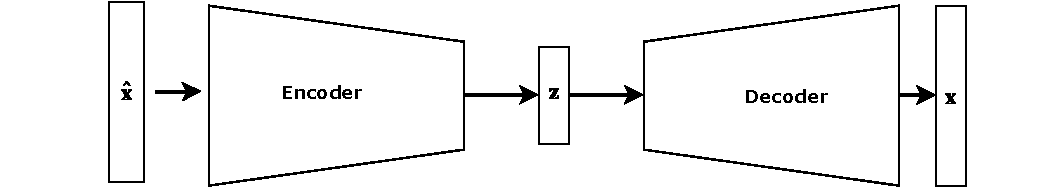
\includegraphics[width=0.8\linewidth]{../chapters/theory/autoencoder/plots/autoencoder.pdf}
		\caption{Autoencoder neural network schematic}%
		\label{fig:autoenc}
	\end{figure}

	An autoencoder is defined by an encoder/decoder pair of neural networks. We construct these such that 
	\begin{align}
		\text{dim}(\mathbf{\hat{x}}) \gg \text{dim}(\mathbf{z}),
	\end{align}

	and with the optimization objective
	\begin{align}
		\mathcal{O} = \text{arg min} || \mathbf{\hat{x}} - \text{Decoder}(\text{Encoder}(\mathbf{\hat{x}}))||_2 ^2.
	\end{align}
\end{frame}

\note{
	\begin{itemize}
		\item Recall that we want to separate classes of reaction products
		\item Additionally - we assume that we have access to very little or no ground truth labelled data
	\end{itemize}
	\begin{block}{ Idea }
		Learn the distribution over the events through two nonlinear maps which compress and inflate a representation of the events.
	\end{block}
	\begin{block}{Central Hypothesis}
		If we can create a compressed representation of an event from which we can reconstruct the event - the compression should be informative\footcite{Fertig} of the type of event that occurred.
	\end{block}
}
\begin{frame}[t]{Applied algorithms}
	Algorithms used from packages:
	\begin{enumerate}[I]
		\item Logistic Regression
		\item K-means clustering
	\end{enumerate}
	Available architectures in code
	\begin{enumerate}[I]
		\item Ordinary Convolutional Autoencoder
		\item Variational Autoencoder ($\beta$, MMD)
		\item Mixture of Autoencoders 
		\item Deep Convolutional Embedded Clustering
	\end{enumerate}
\end{frame}

\begin{frame}[t]{Experiment}
	\begin{itemize}
		\item We chose to represent the data as 2D projections.
		\item An autoencoder network is then fit.
		\item After traing, we extract the compressed (or \textit{latent}) expressions.
		\item With varying amounts of labelled ground-truth data we fit a very simple classifier to the latent expressions.
	\end{itemize}
	We wish to construct latent spaces that are as close to trivially separable, and so use a logistic regression classifier.
\end{frame}


\note{
	\begin{itemize}
		\item Neglecting the z-axis.
		\item autoencoder is fit events in an end to end manner.
		\item of the data
		\item With varying amounts of labelled ground-truth data we fit a very simple classifier to the latent expressions
	\end{itemize}
}

\begin{frame}[t]{Results}
	\begin{figure}[h]
		\subfloat[Convolutional autoencoder performance with a naive architecture]{\includegraphics[height=3.5cm]{../chapters/results/classification/plots/ac_n_samples.pdf}}
		\subfloat[Convolutional autoencoder performance using a VGG16 representation representation of the events.]{\includegraphics[height=3.5cm]{../chapters/results/classification/plots/vgg_ac_n_samples.pdf}}
	\end{figure}
\end{frame}

\note{
Most important region is the left-most side of the plot, with few samples
}

\begin{frame}[t]{Clustering}
	\begin{itemize}
		\item We demonstrated that we can construct high quality spaces that are linearly separable
		\item The next step then is a \textit{clustering} task. Can we separate classes without knowing the ground truth labels? 
	\end{itemize}
	We explored two autoencoder-based clustering algorithms, in addition to ordinary K-means clustering.
\end{frame}

\note{
	Clustering, while similar to classification have some principal differences.
}

\begin{frame}[t]{K-means clustering}
	\begin{itemize}
		\item Ordinary K-means on the two-dimensional representations would obviously not be productive because of the dimensionality of the problem.
		\item Instead we try to cluster the representation of the events as seen by an image classifying algorithm: VGG16
	\end{itemize}

	With $8e3$ output nodes the VGG16 representation is still very much high dimenisonal, but importantly it is sparse.
\end{frame}

\begin{frame}[t]{K-means results}
	\begin{figure}[h]
		\centering
		\subfloat{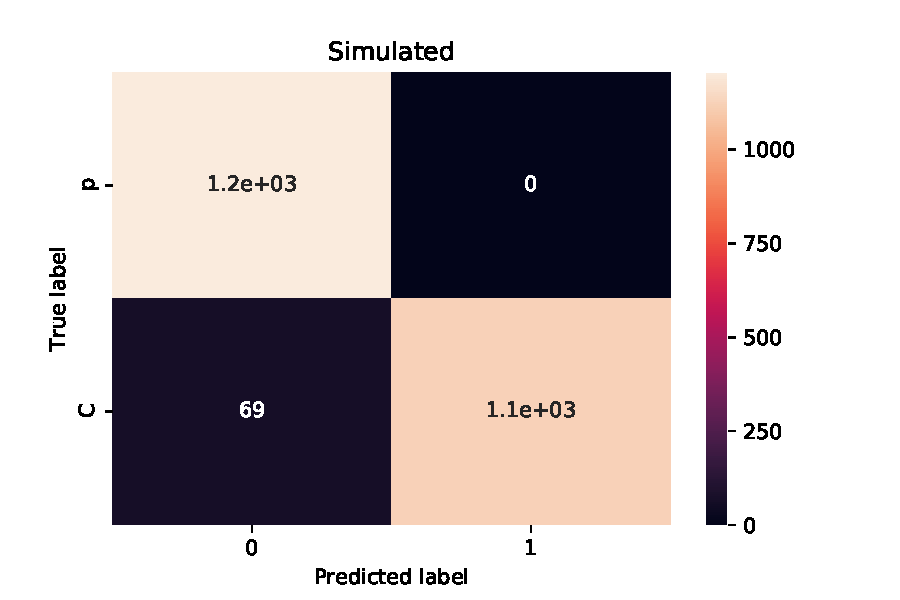
\includegraphics[width=0.35\textwidth]{../chapters/results/clustering/plots/Simulatedvgg_pca_conf_mat.pdf}}
		\subfloat{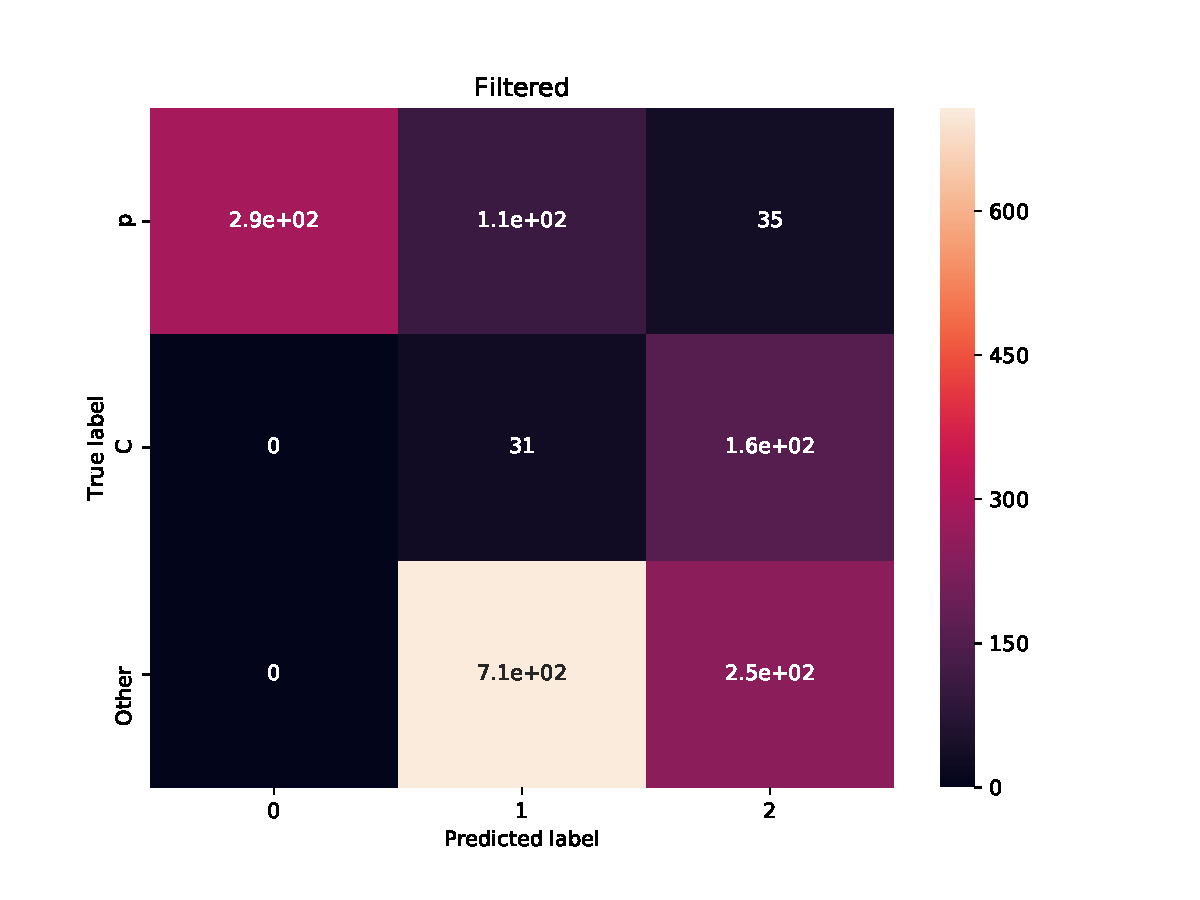
\includegraphics[width=0.35\textwidth]{../chapters/results/clustering/plots/Filteredvgg_pca_conf_mat.pdf}}
		\subfloat{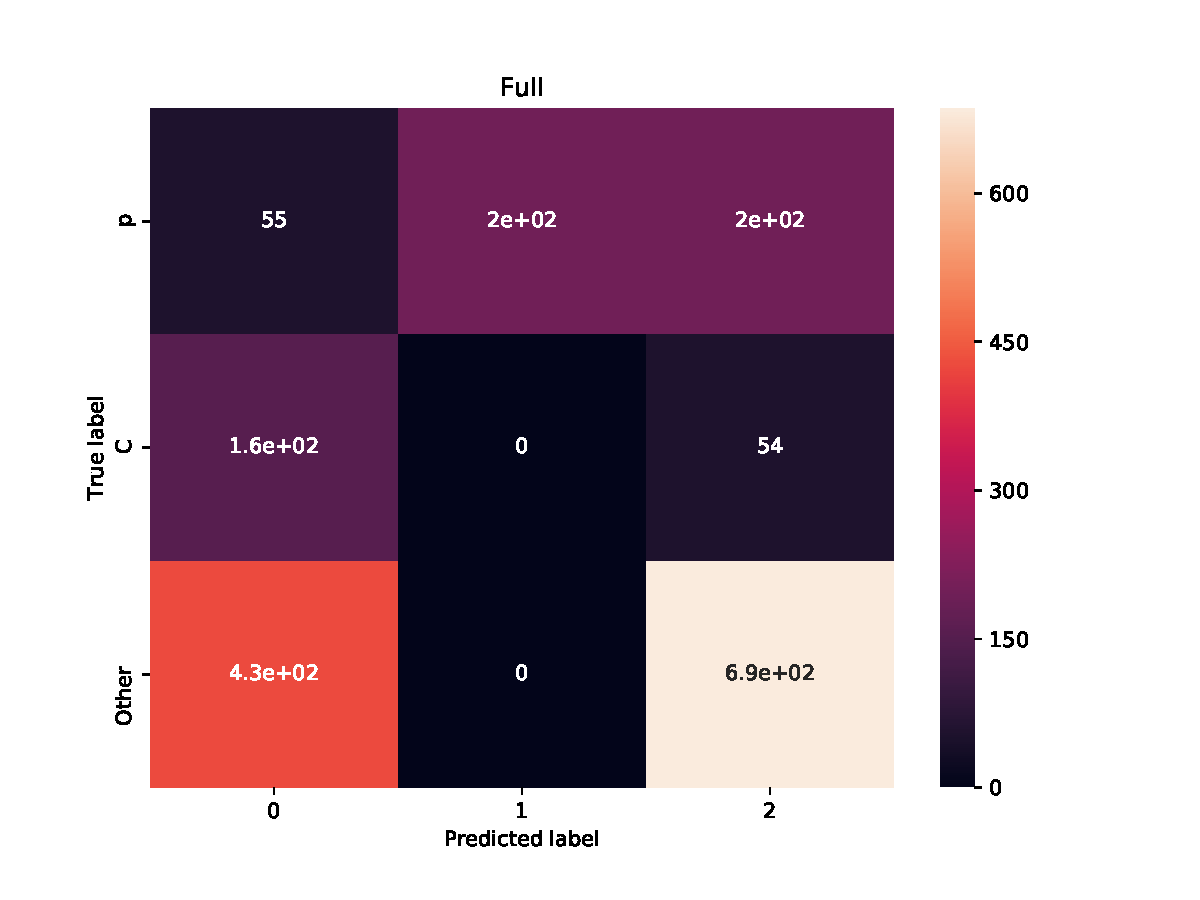
\includegraphics[width=0.35\textwidth]{../chapters/results/clustering/plots/Fullvgg_pca_conf_mat.pdf}}
		\caption{K-means clustering results using the VGG16 representation of the datasets}
	\end{figure}
	Cluster elements for clustering full data 
	\centering 
	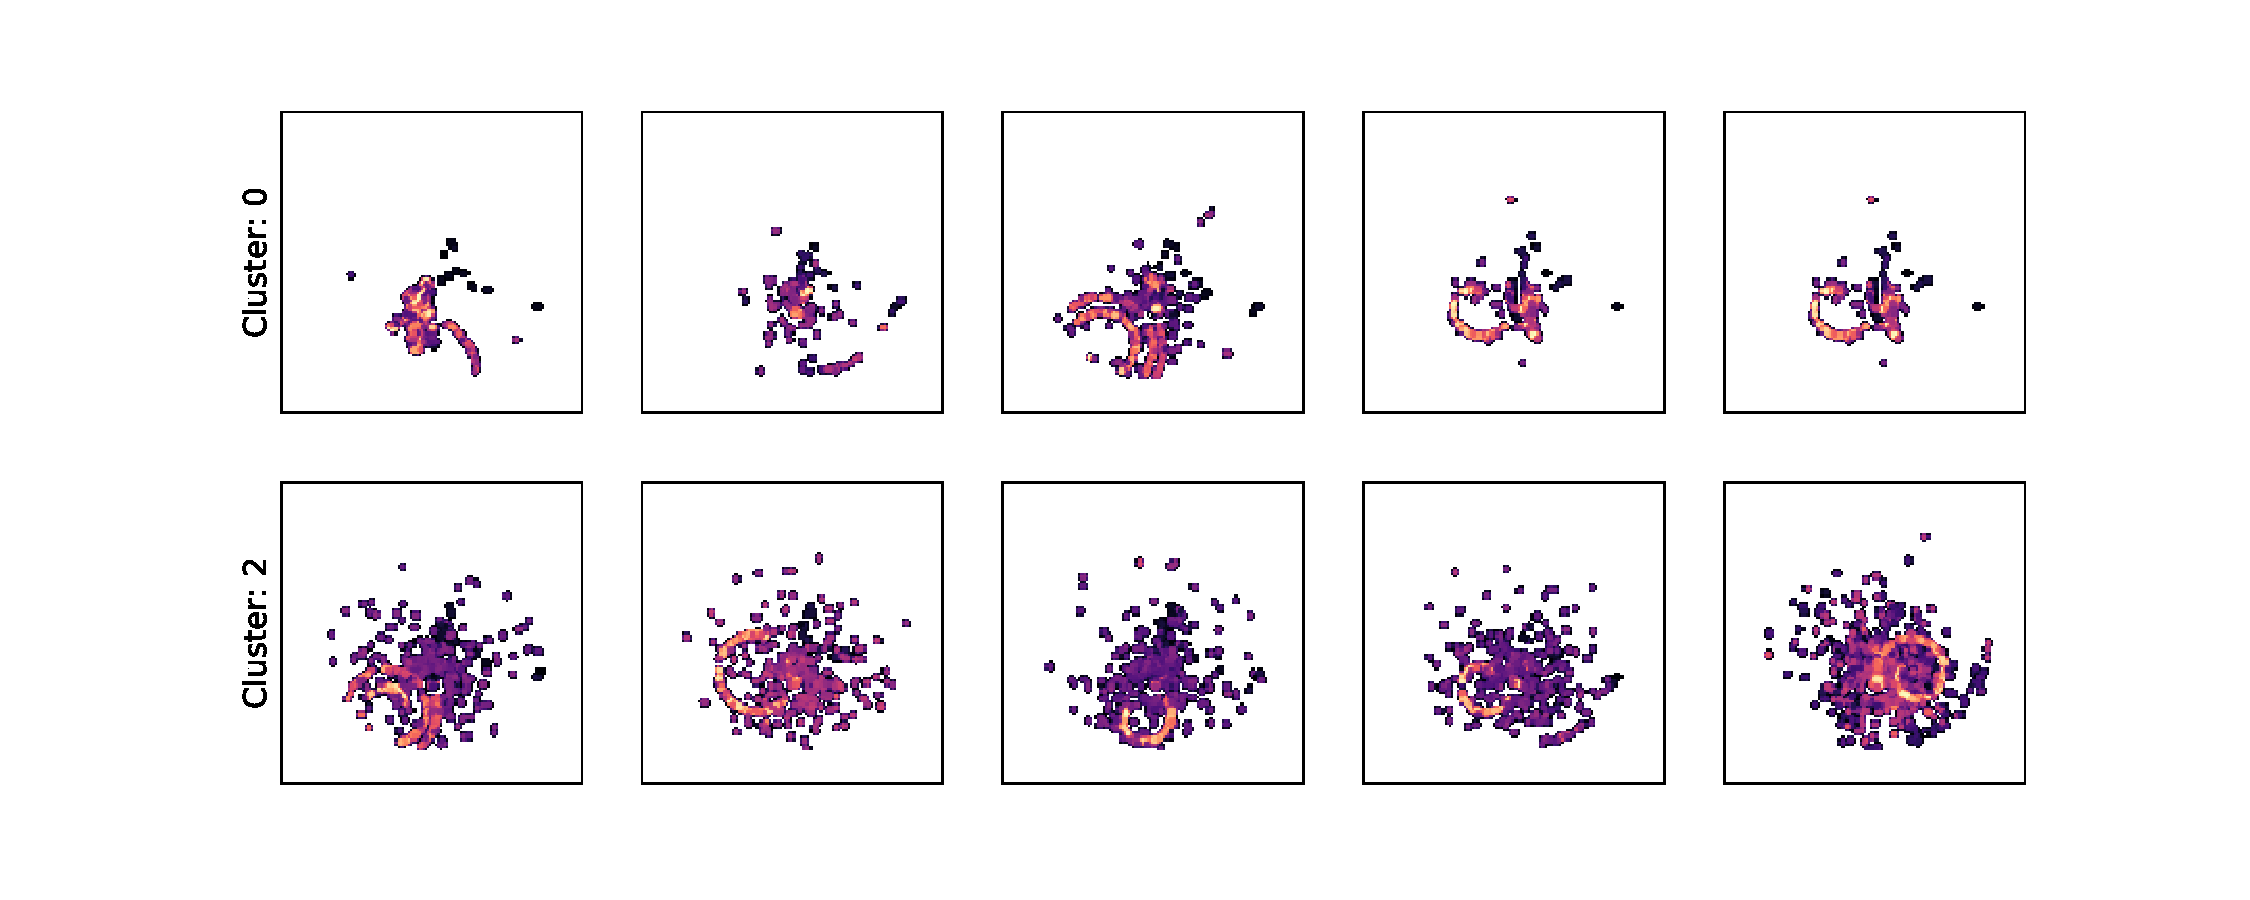
\includegraphics[height=3cm]{../chapters/results/clustering/plots/full_vgg_cluster_repr.pdf}
\end{frame}

\note{
	Clusters are well defined if they have one cell along the vertical axis. \\
	And perfect if they are empty in a cross
}

\begin{frame}[t]{Mixture of Autoencoders}
	\begin{itemize}
		\item One can also attempt clustering with Autoencoder based algorithms
		\item Niche field with only limited applications (MNIST, Reuters)
	\end{itemize}

	\centering
	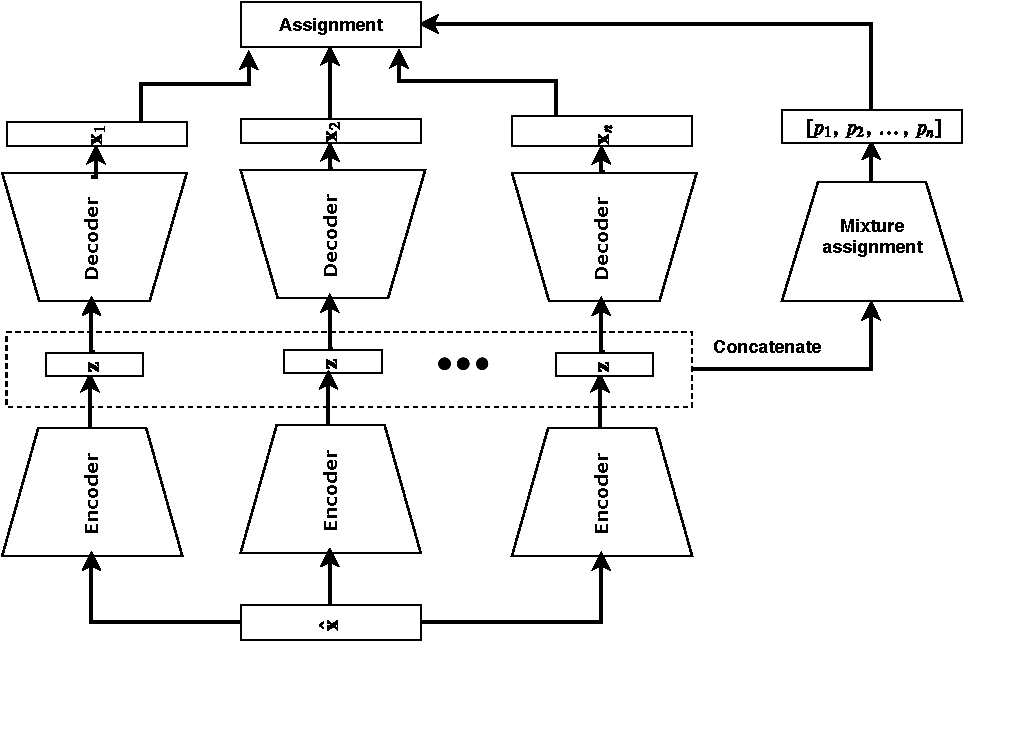
\includegraphics[height=6cm]{../chapters/theory/autoencoder/plots/mixae.pdf}
\end{frame}


\begin{frame}[t]{Deep Clustering Results}
	\centering 
	\begin{figure}[h]
		\subfloat{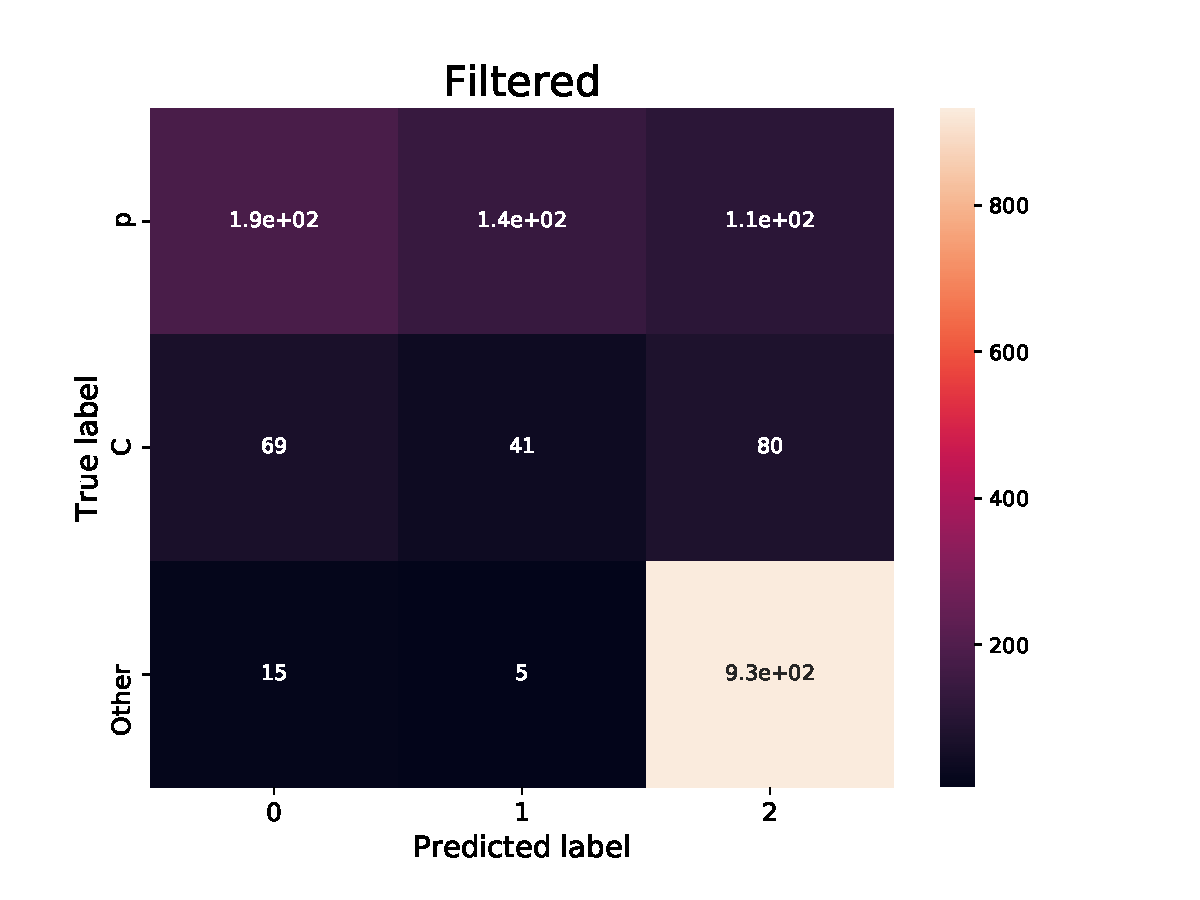
\includegraphics[width=5cm]{../chapters/results/clustering/plots/Filtered_mixae_conf_mat.pdf}}
		\subfloat{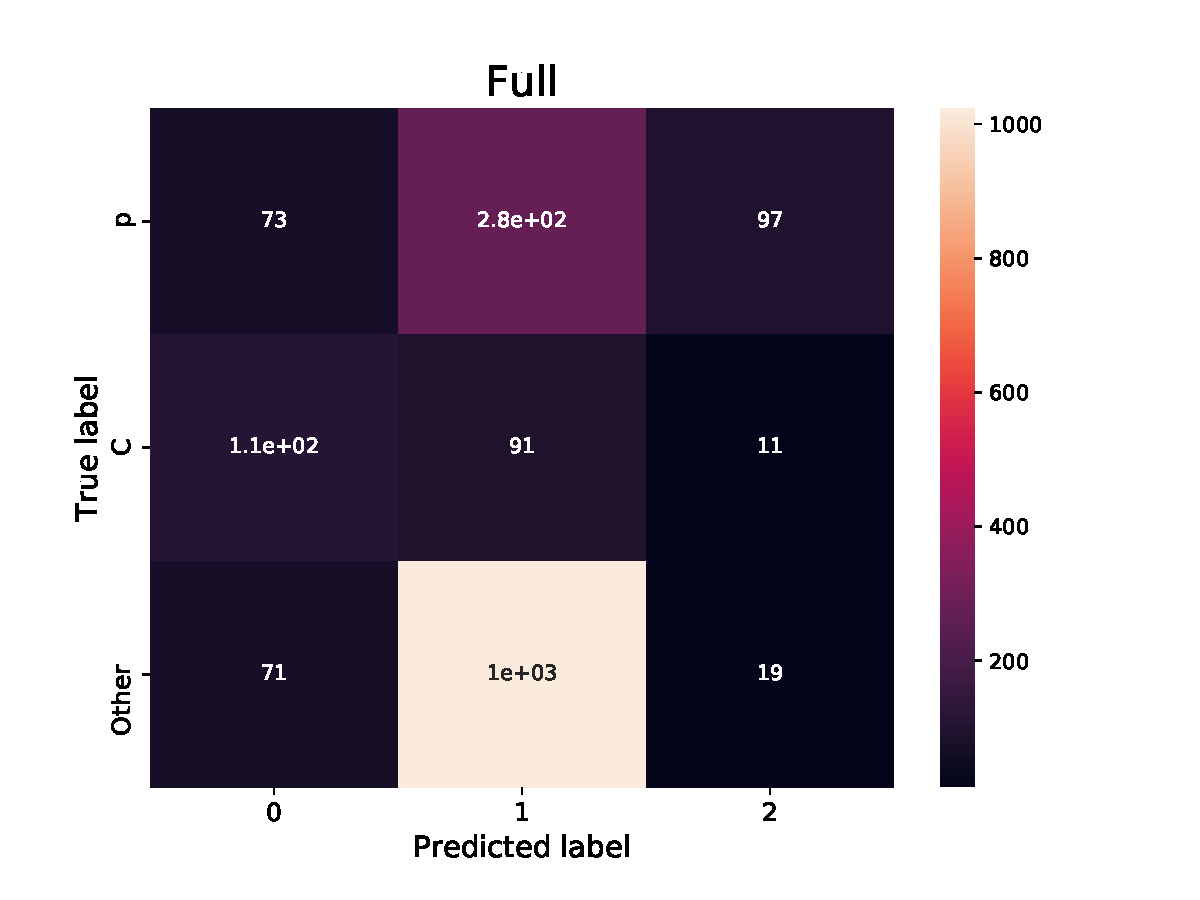
\includegraphics[width=5cm]{../chapters/results/clustering/plots/full_mixae_conf_mat.pdf}}
		\caption{Top-performing mixae results for the real experimental data}
	\end{figure}
	Cluster elements for clustering of full data
	
\includegraphics[height=3cm]{../chapters/results/clustering/plots/real_cluster_repr.pdf}
\end{frame}

\note{
	Plagued by instability even with the same hyperparameters
	Remember to link the plots together
}

\begin{frame}[t]{Summary and Outlook}
	\begin{itemize}
		\item We have shown that Autoencoder models are suitable for both semi-supervised and unsupervised applications.
		\item Autoencoder clustering has a fundamental challenge with issues of stability and convergence. We still need labelled samples to verify.
		\item Including physical parameters increases the quality of the latent space.
	\end{itemize}
	Neural network models clearly have a place in this analyisis going forward: but connecting the anlysis to the physical properties of the system remains a challenge to solve.
\end{frame}

\begin{frame}[t]{AT-TPC pad plane}
	\begin{figure}
		\centering
		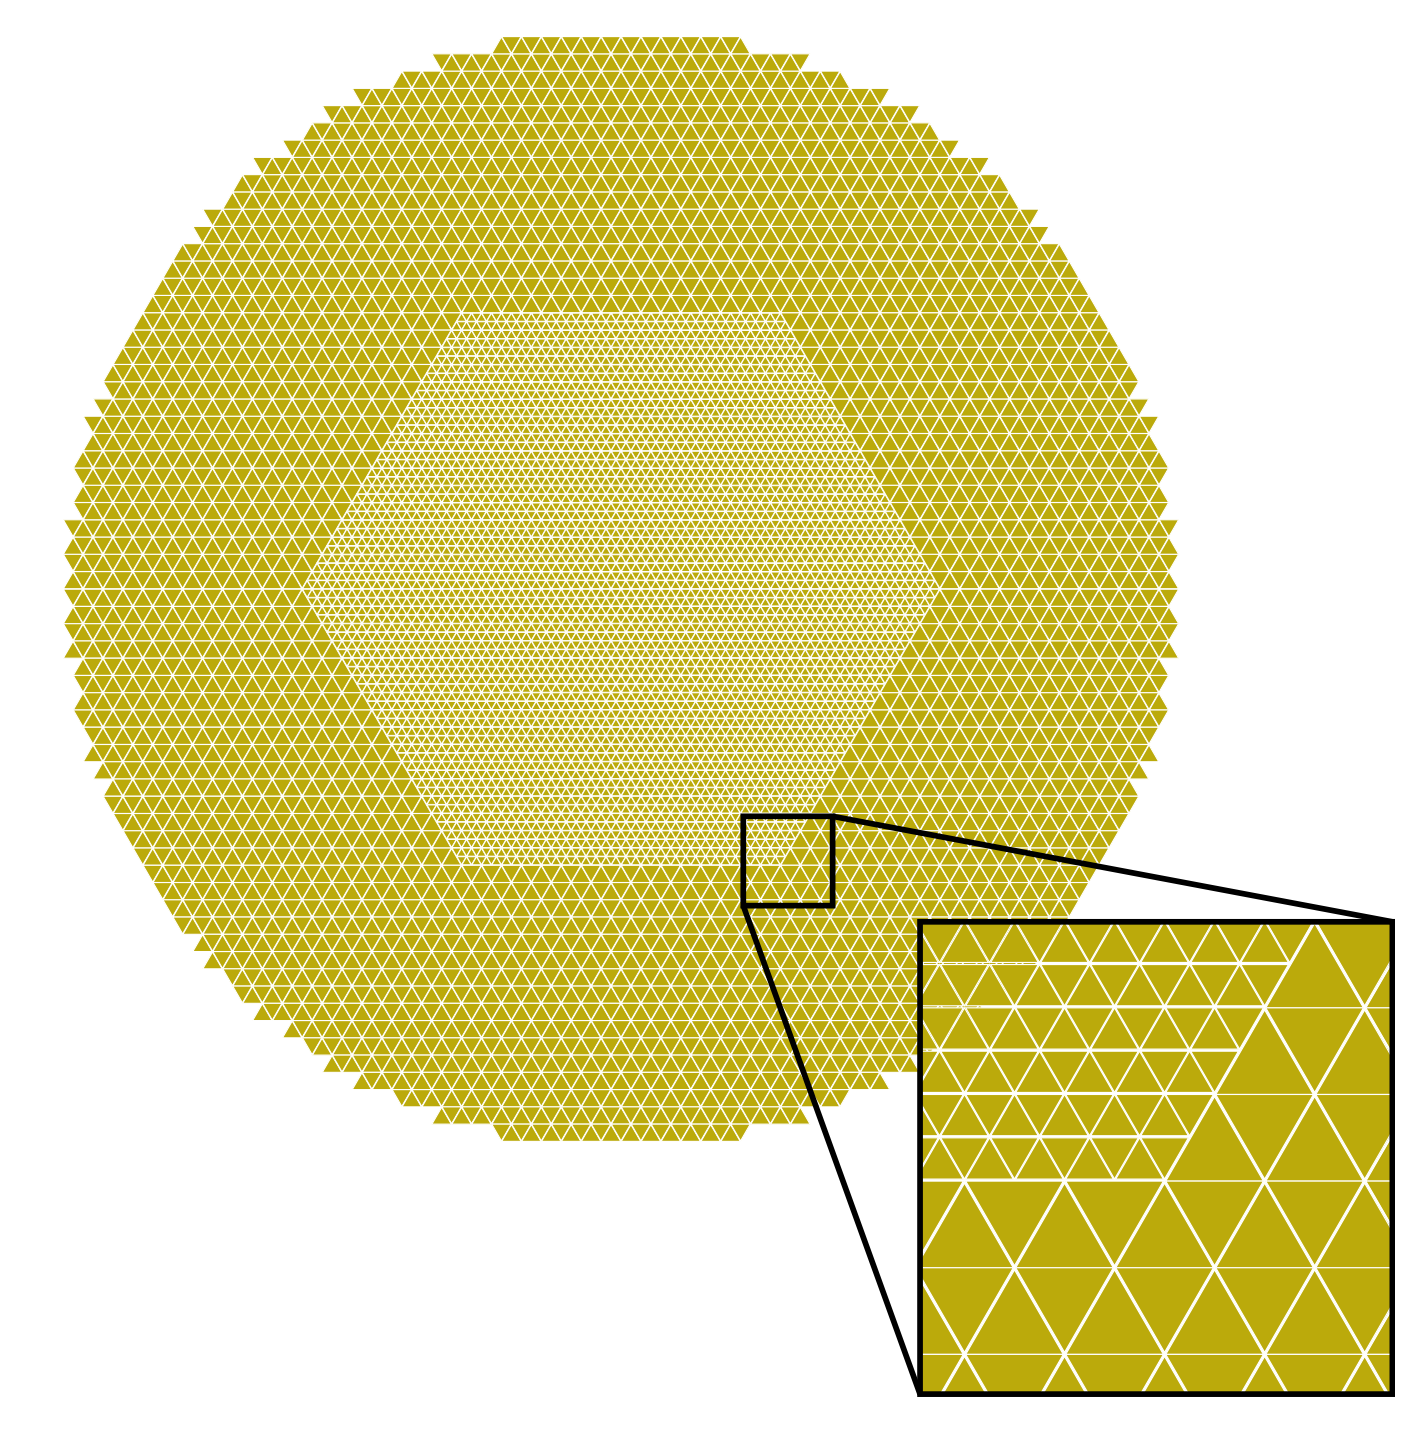
\includegraphics[height=3cm]{../chapters/experimental_background/plots/at_tpc_padplane.png}
		\caption{Detector pad plane of the AT-TPC \footcite{Bradt2017a}}\label{fig:padplane}
	\end{figure}
	Each triangle represents spatial discrete regions of the detector surface. The pad-plane consists of some $10^4$ sensor pads on a circle with $r=29cm$
\end{frame}


\begin{frame}[t]{f1 score}
	\begin{equation}\label{eq:recall}
	\text{recall}= \frac{TP}{TP + FP}, \quad
	\text{precision} = \frac{TP}{TP + FN}.
	\end{equation}

	\noindent The $f1$ score is defined as the harmonic mean of precision and recall for each class. Formally we define it as

	\begin{equation}\label{eq:f1}
	f1 = 2 \frac{\text{precision} \cdot \text{recall}}{\text{precision} + \text{recall}}.
	\end{equation}
\end{frame}

\begin{frame}[t]{Bias-variance decomposition}
	\begin{figure}[h]
		\centering
		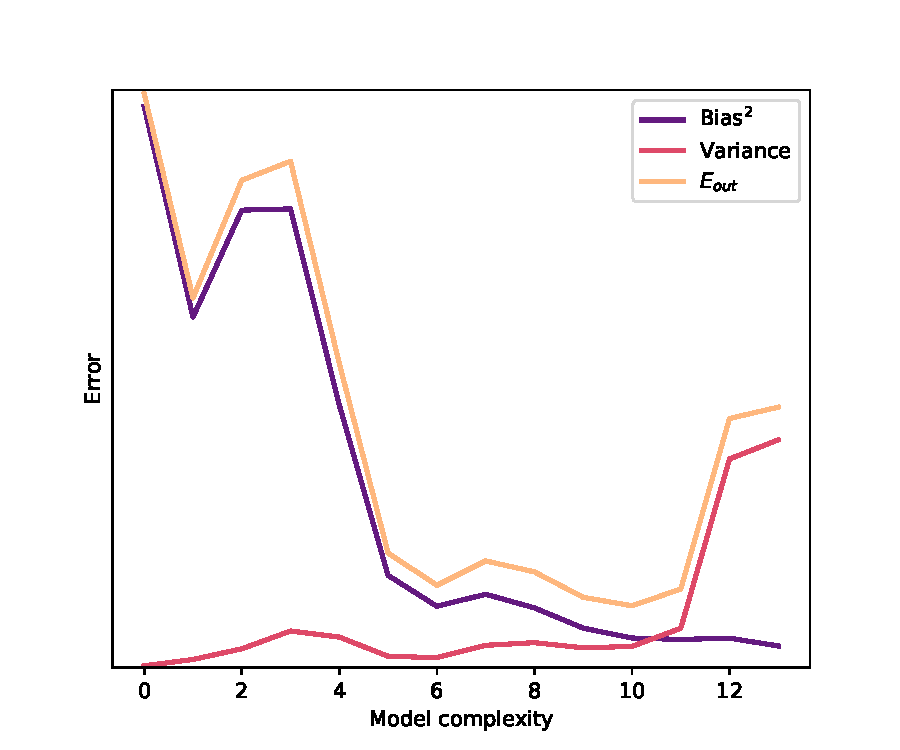
\includegraphics[width=0.55\linewidth]{../chapters/theory/figures/bias_var_degree.pdf}
		\caption{Bias - variance decomposition of the MSE objective with iid. noise. Generalization error is denoted $E_{out}$, and is the sum of the Bias and Variance terms.}
		\label{fig:bv}
	\end{figure}
	The quality of a model is measured by how well it does on data not seen during training, measured by $E_{out}$.
\end{frame}

\begin{frame}[t]{Implementing details}
	Models implemented in Python with TensorFlow (TF), a ML framework developed by Google.
	TensorFlow provided a base on which to build complex NN models.
	Code written for this analyis includes 

	\begin{enumerate}[I]
		\item Abstraction for autoencoder networks,
		\item Implementation of variations on the Variational Autoencoder,
		\item Custom class implementations based on the high-level Keras API for deep clustering.
	\end{enumerate}
\end{frame}

\begin{frame}[t]{Instability in clustering training}
\centering 
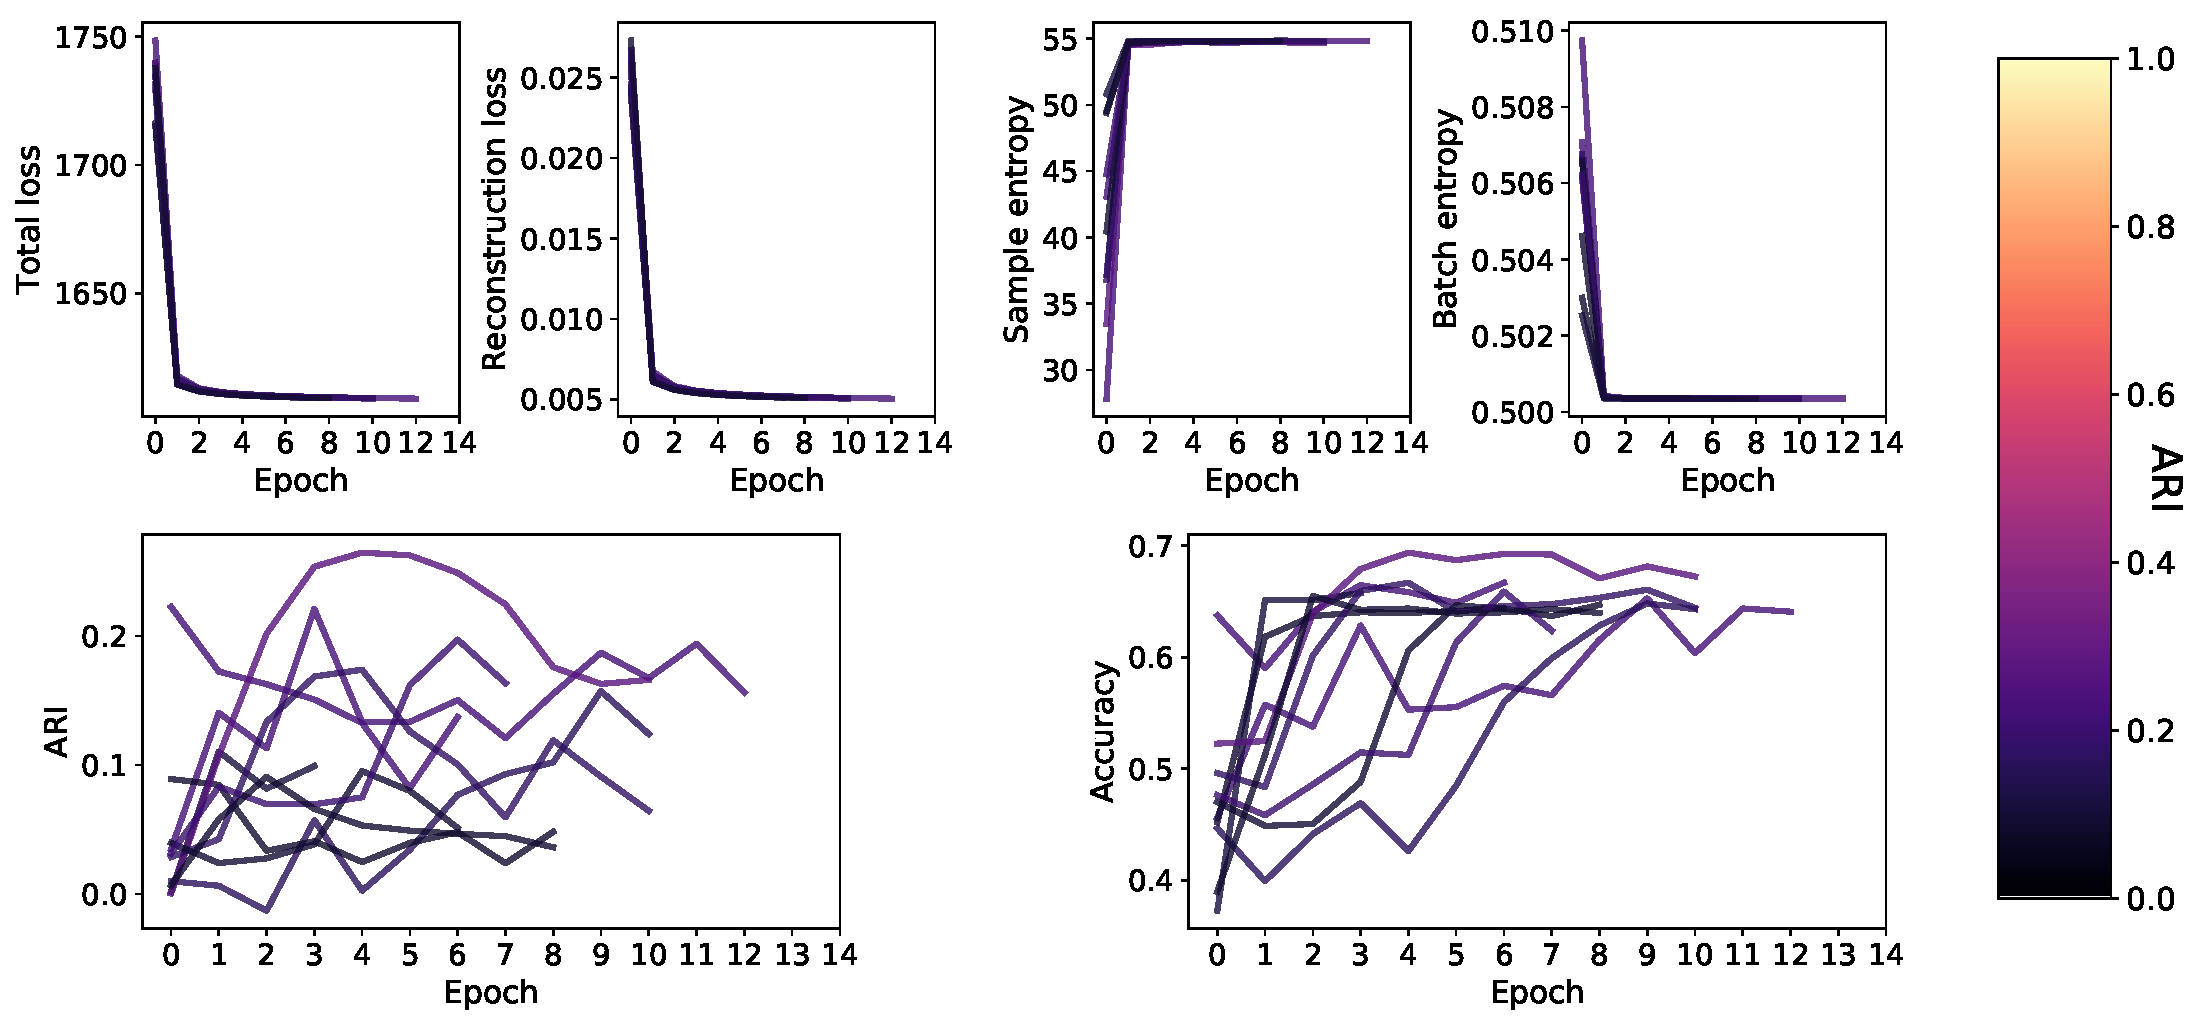
\includegraphics[width=\textwidth]{../chapters/results/clustering/plots/real_mixae.pdf}
Several runs with the same hyperparameters.
\end{frame}

\note{
	Perhaps the most curious result, not only the instability but the high Sample Entropy.
}
\end{document}

